\documentclass{beamer}

\usepackage[russian]{babel}
\usepackage[utf8]{inputenc}
\usepackage{cmap}
\usepackage{graphicx}
\usepackage{xspace}
\usepackage{psfrag}
\usepackage{float}

\newcommand{\MARK}[1]{{\bf {\it #1}}}
\newcommand{\CODE}[1]{{\ttfamily #1}}

\setbeamertemplate{footline}[frame number]
\usecolortheme{seahorse}
\beamertemplateshadingbackground{white}{blue!3}

\begin{document}
\sloppy

\begin{frame}
\begin{center}
Жарков Денис\\
\vspace{1cm}
{\Large Реализация системы генерации статистических отчетов для IPTV провайдера}
\end{center}
\begin{tabbing}
\hspace{6.5cm} \= Научный руководитель\\
\> Приступа П.В.\\
\end{tabbing}
\end{frame}

\begin{frame}
\frametitle{IPTV провайдер}
Организация, предоставляющая доступ к media-контенту абонентам в сетях передачи данных по протоколу IP
\\
\vspace{0.3cm}
{\bf Функции}
\begin{itemize}
\item{
Заключение договоров с правообладателями
}
\item{
Предоставление абонентам услуг IPTV и VOD (Video On Demand)
}
\end{itemize}
\end{frame}

\begin{frame}
\frametitle{Задачи}
\begin{enumerate}
\item {
Импорт данных
}
\item {
Реализация удобного интерфейса для поиска, просмотра и редактирования данных.
}
\item {
Расчет отчислений по LIVE
}
\item {
Генерация отчетов по LIVE и VOD
}
\item {
Разграничение прав доступа
}
\end{enumerate}
\end{frame}

\begin{frame}
\frametitle{Реализация}

Система реализована в виде веб-приложения\\
В качестве основной среды разработки был выбран фреймворк Yii (PHP),\\
а в качестве хранилища данных --- СУБД Microsoft SQL Server.\\

\end{frame}

\begin{frame}[t]
\frametitle{Реализация. Модель БД для Live. Отчисления}
\begin{figure}
\begin{center}
\vspace{-1cm}
\hspace*{-1cm} 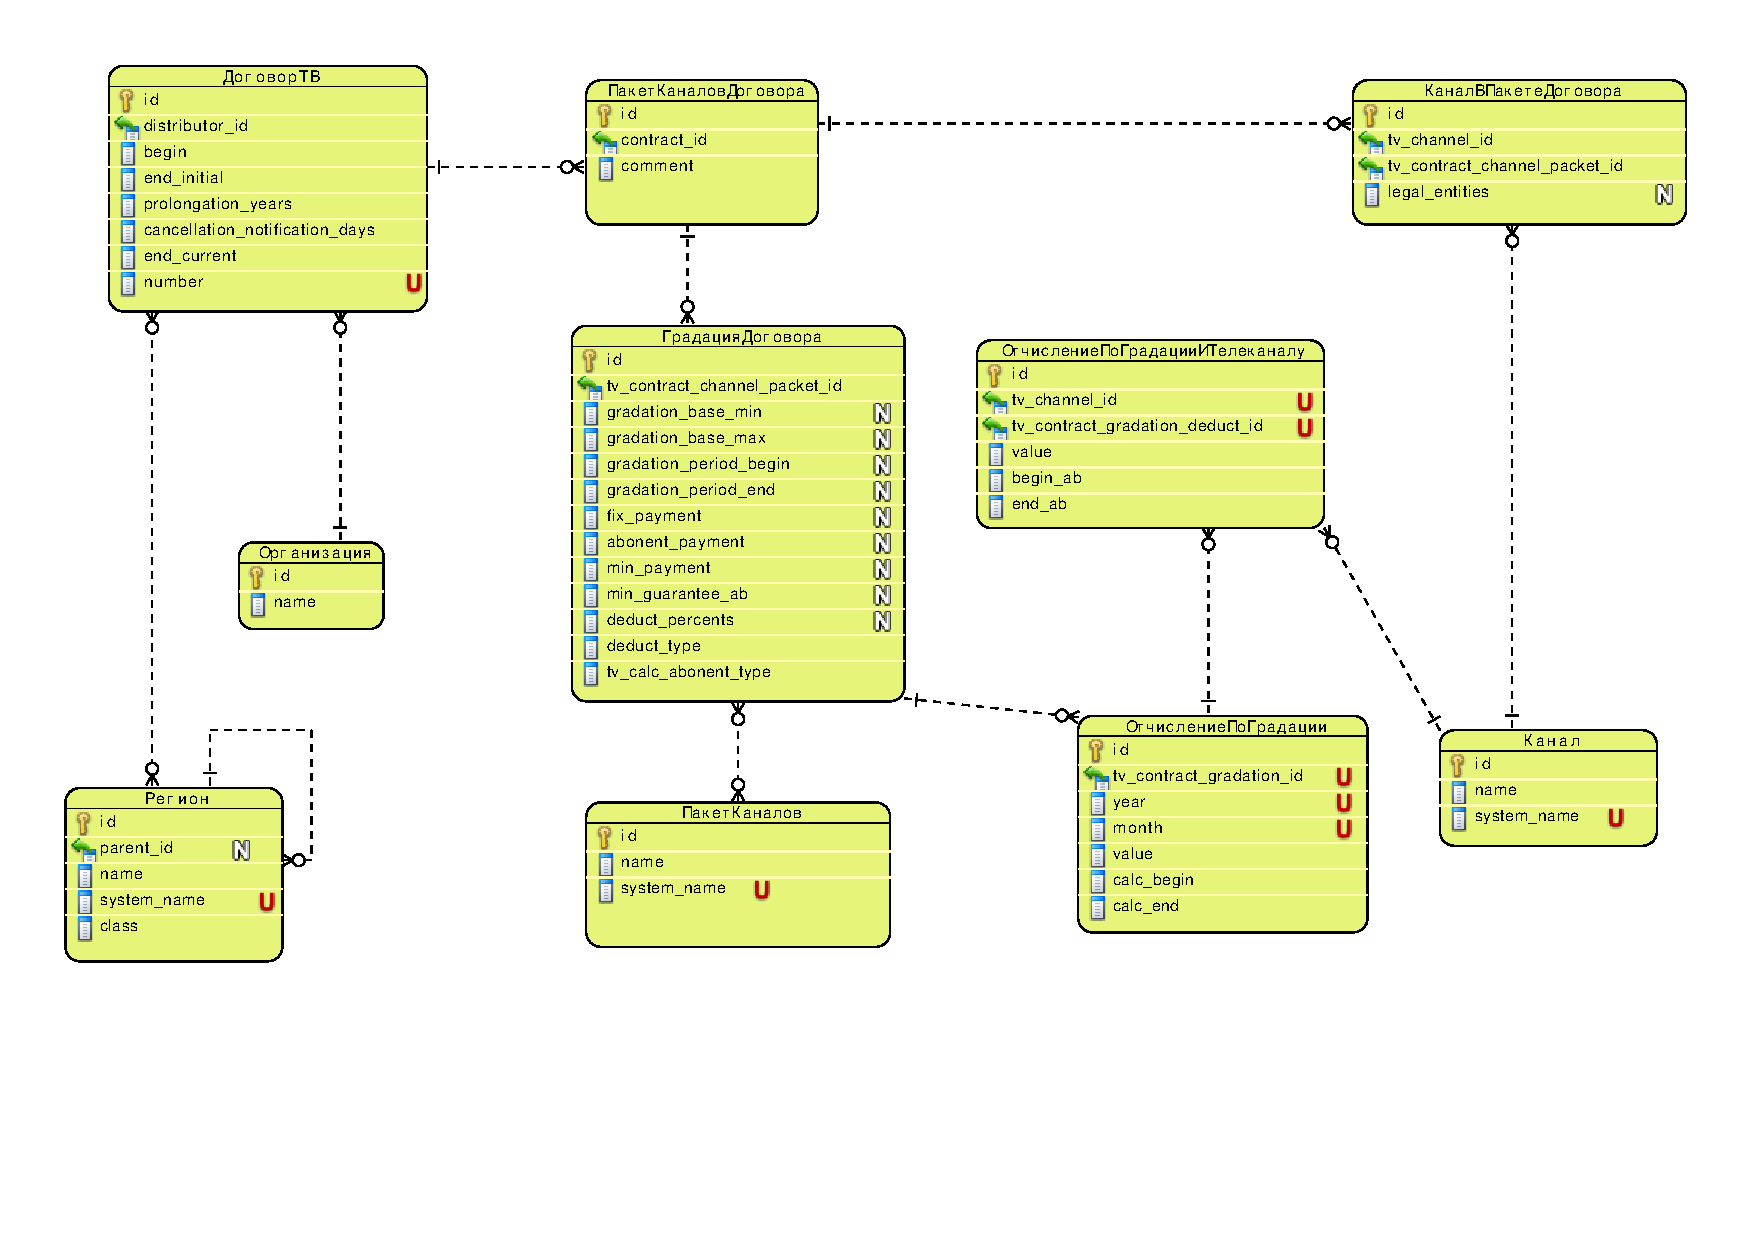
\includegraphics[scale=0.43]{../resources/uml/TV_DEDUCT.pdf}
\end{center}
\end{figure}
\end{frame}

\begin{frame}[t]
\frametitle{Реализация. Модель БД для Live. Статистика}
\begin{figure}
\begin{center}
\vspace{-1cm}
\hspace*{-1cm} 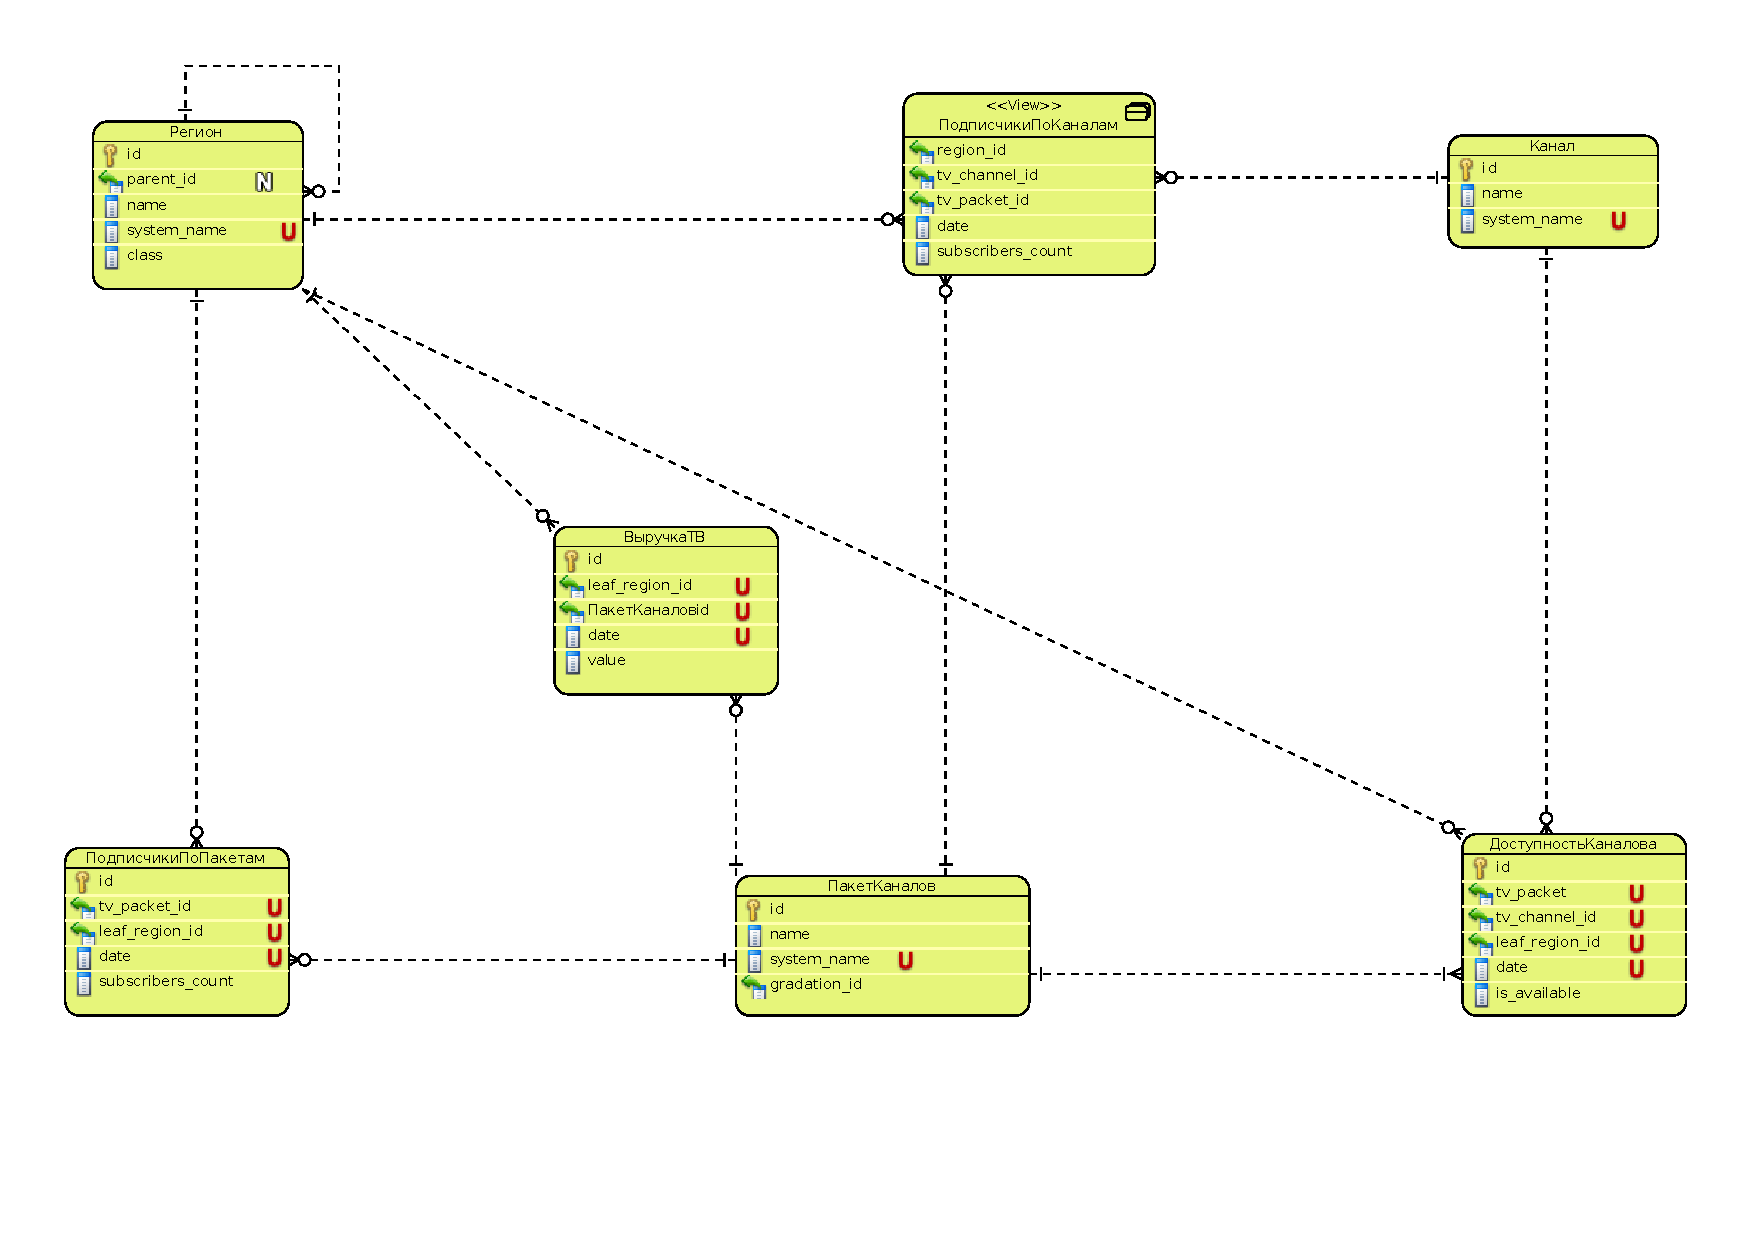
\includegraphics[scale=0.43]{../resources/uml/TV_STAT.pdf}
\end{center}
\end{figure}
\end{frame}

\begin{frame}[t]
\frametitle{Реализация. Модель БД для VOD. Отчисления}
\begin{figure}
\begin{center}
\vspace{-1cm}
\hspace*{-1cm} 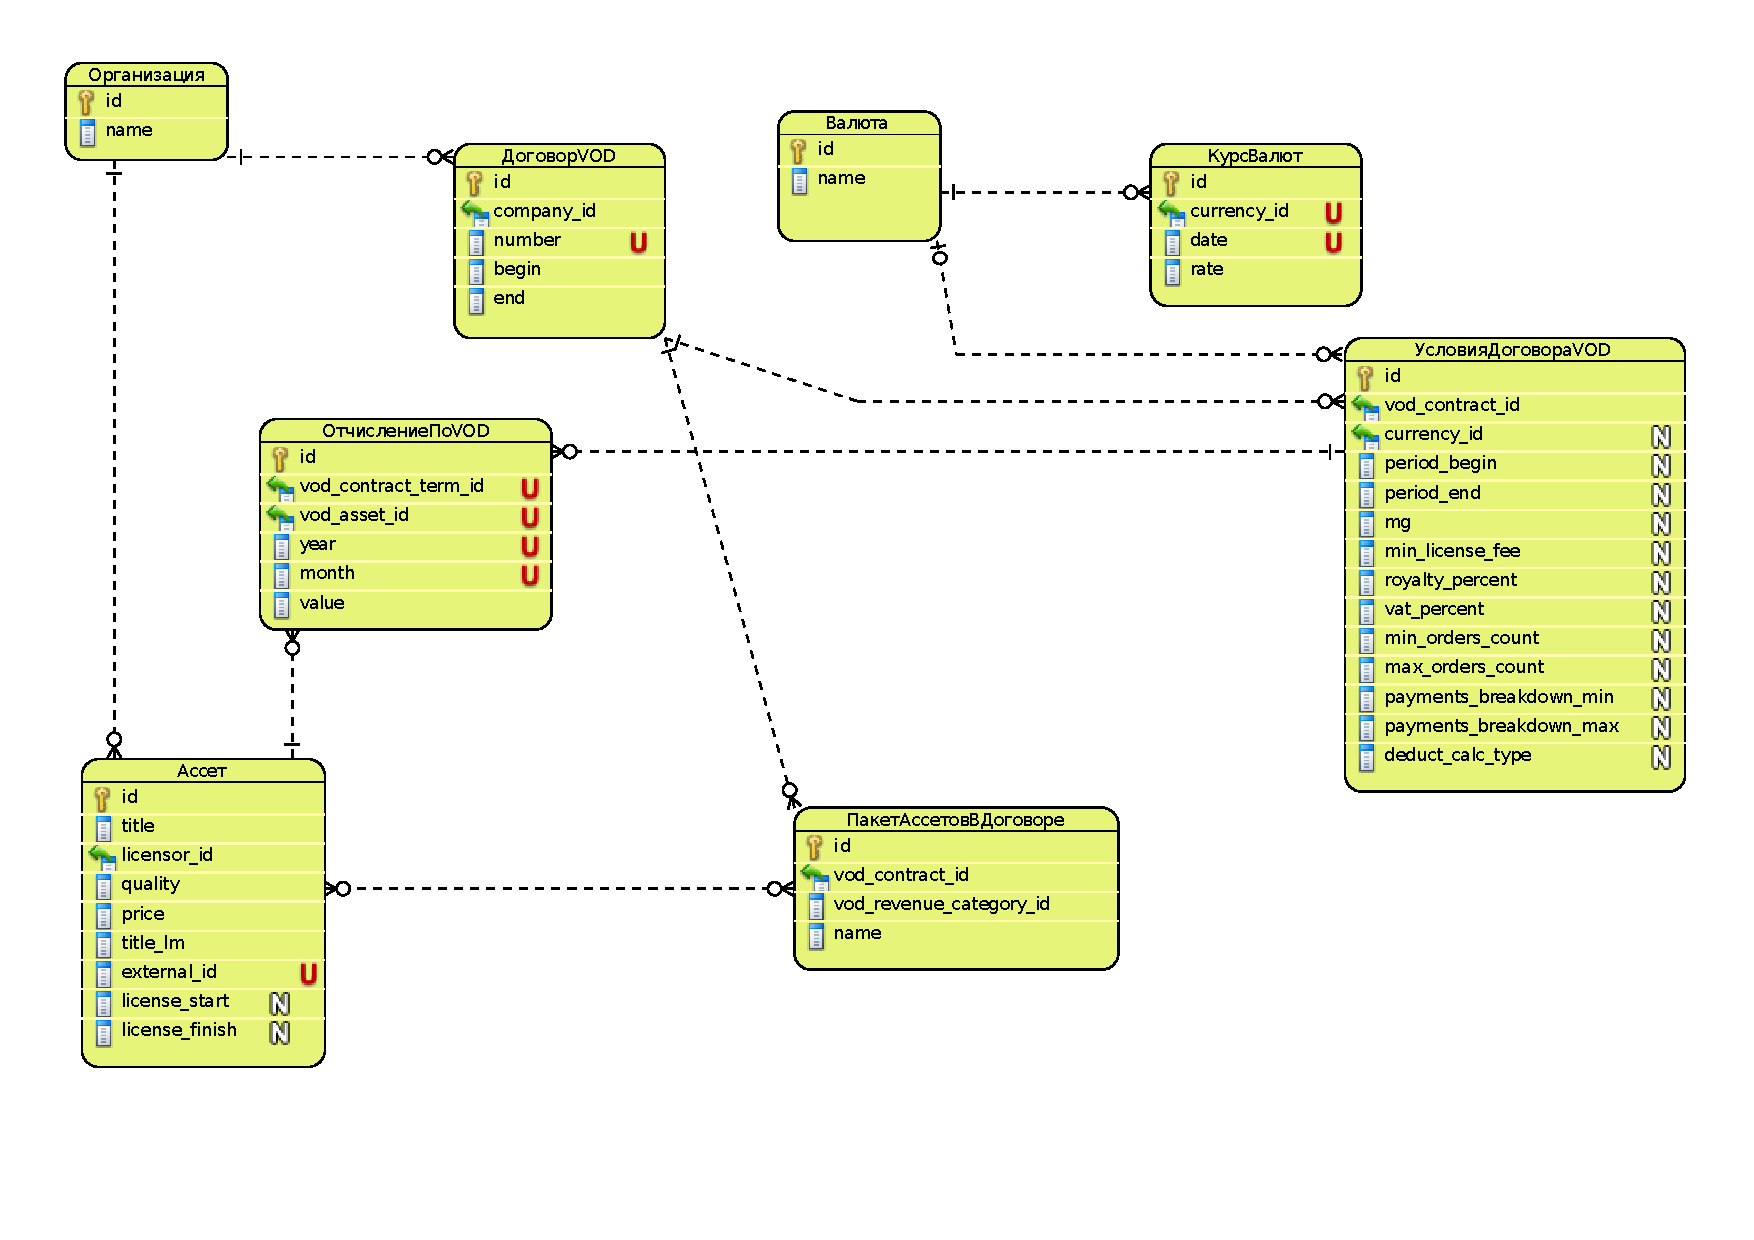
\includegraphics[scale=0.43]{../resources/uml/VOD_DEDUCT.pdf}
\end{center}
\end{figure}
\end{frame}

\begin{frame}[t]
\frametitle{Реализация. Модель БД для VOD. Статистика}
\begin{figure}
\begin{center}
\vspace{1cm}
\hspace*{-1cm} 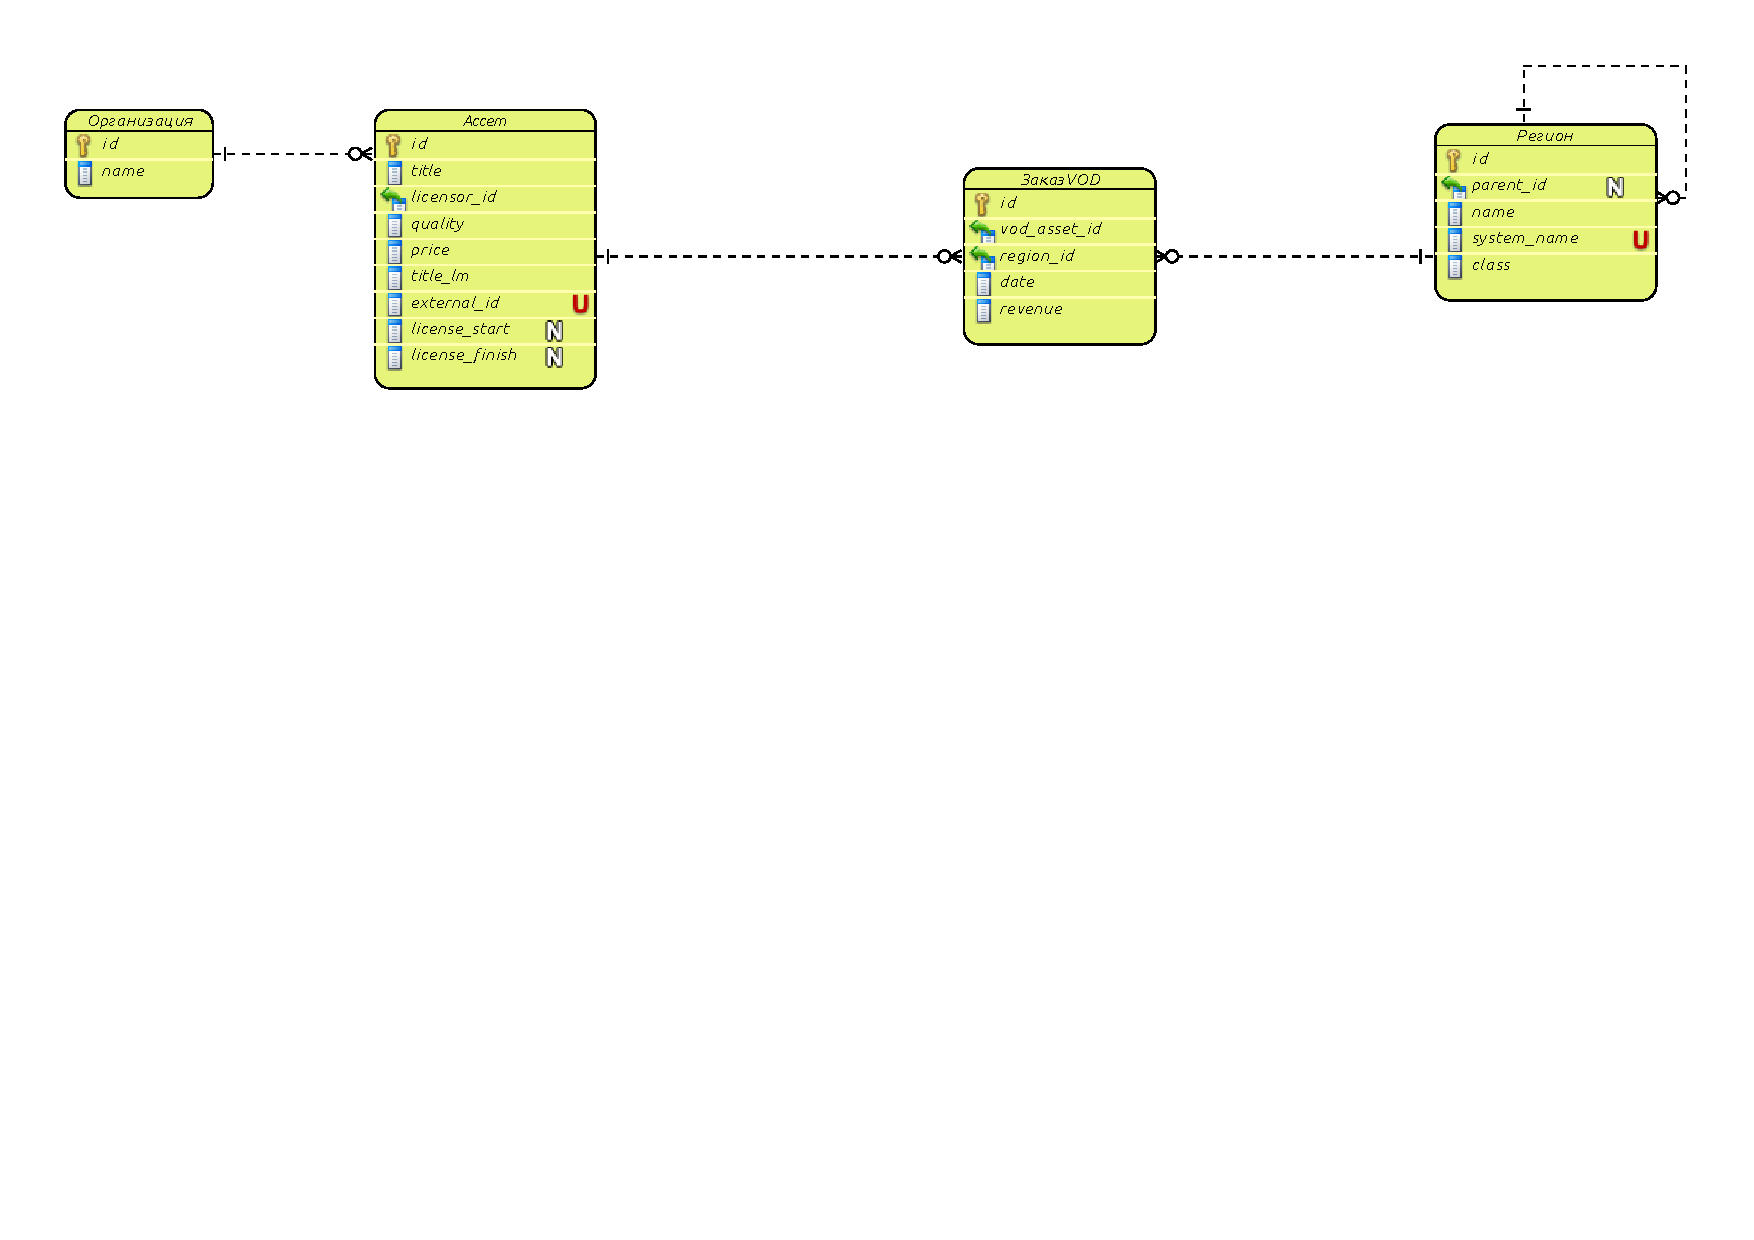
\includegraphics[scale=0.43]{../resources/uml/VOD_STAT.pdf}
\end{center}
\end{figure}
\end{frame}

%\begin{frame}
%\frametitle{Задачи. Импорт данных}
%
%
%\begin{itemize}
%\item{
%  Импорт данных для справочников (регионы, организации, курсы валют)
%}
%\item{
%  Импорт договоров из XLS-файла --- условия предоставления контента правообладателями
%}
%\item{
%  Импорт ассетов для VOD (Mediaroom)
%}
%\item{
%  Импорт статистики из биллинга (XML) --- статистика потребления контента пользователями
%}
%\end{itemize}

%\end{frame}

%\begin{frame}
%\frametitle{Задачи. Расчет отчислений по LIVE}

%\begin{itemize}
%\item{
%  Ежемесячный расчет
%}
%\item{
%  Договора содержат градации (по периоду/по базе абонентов)
%}
%\item{
%  Градации с фиксированным платежом
%}
%\item{
%  Градации с платежом за абонента (с мин. гарантиями)
%}
%\item{
%  Региональность
%}
%\end{itemize}

%\end{frame}

\begin{frame}
\frametitle{Реализация. Отчеты}
\begin{figure}
\vspace{-1cm}
\hspace*{-1cm} 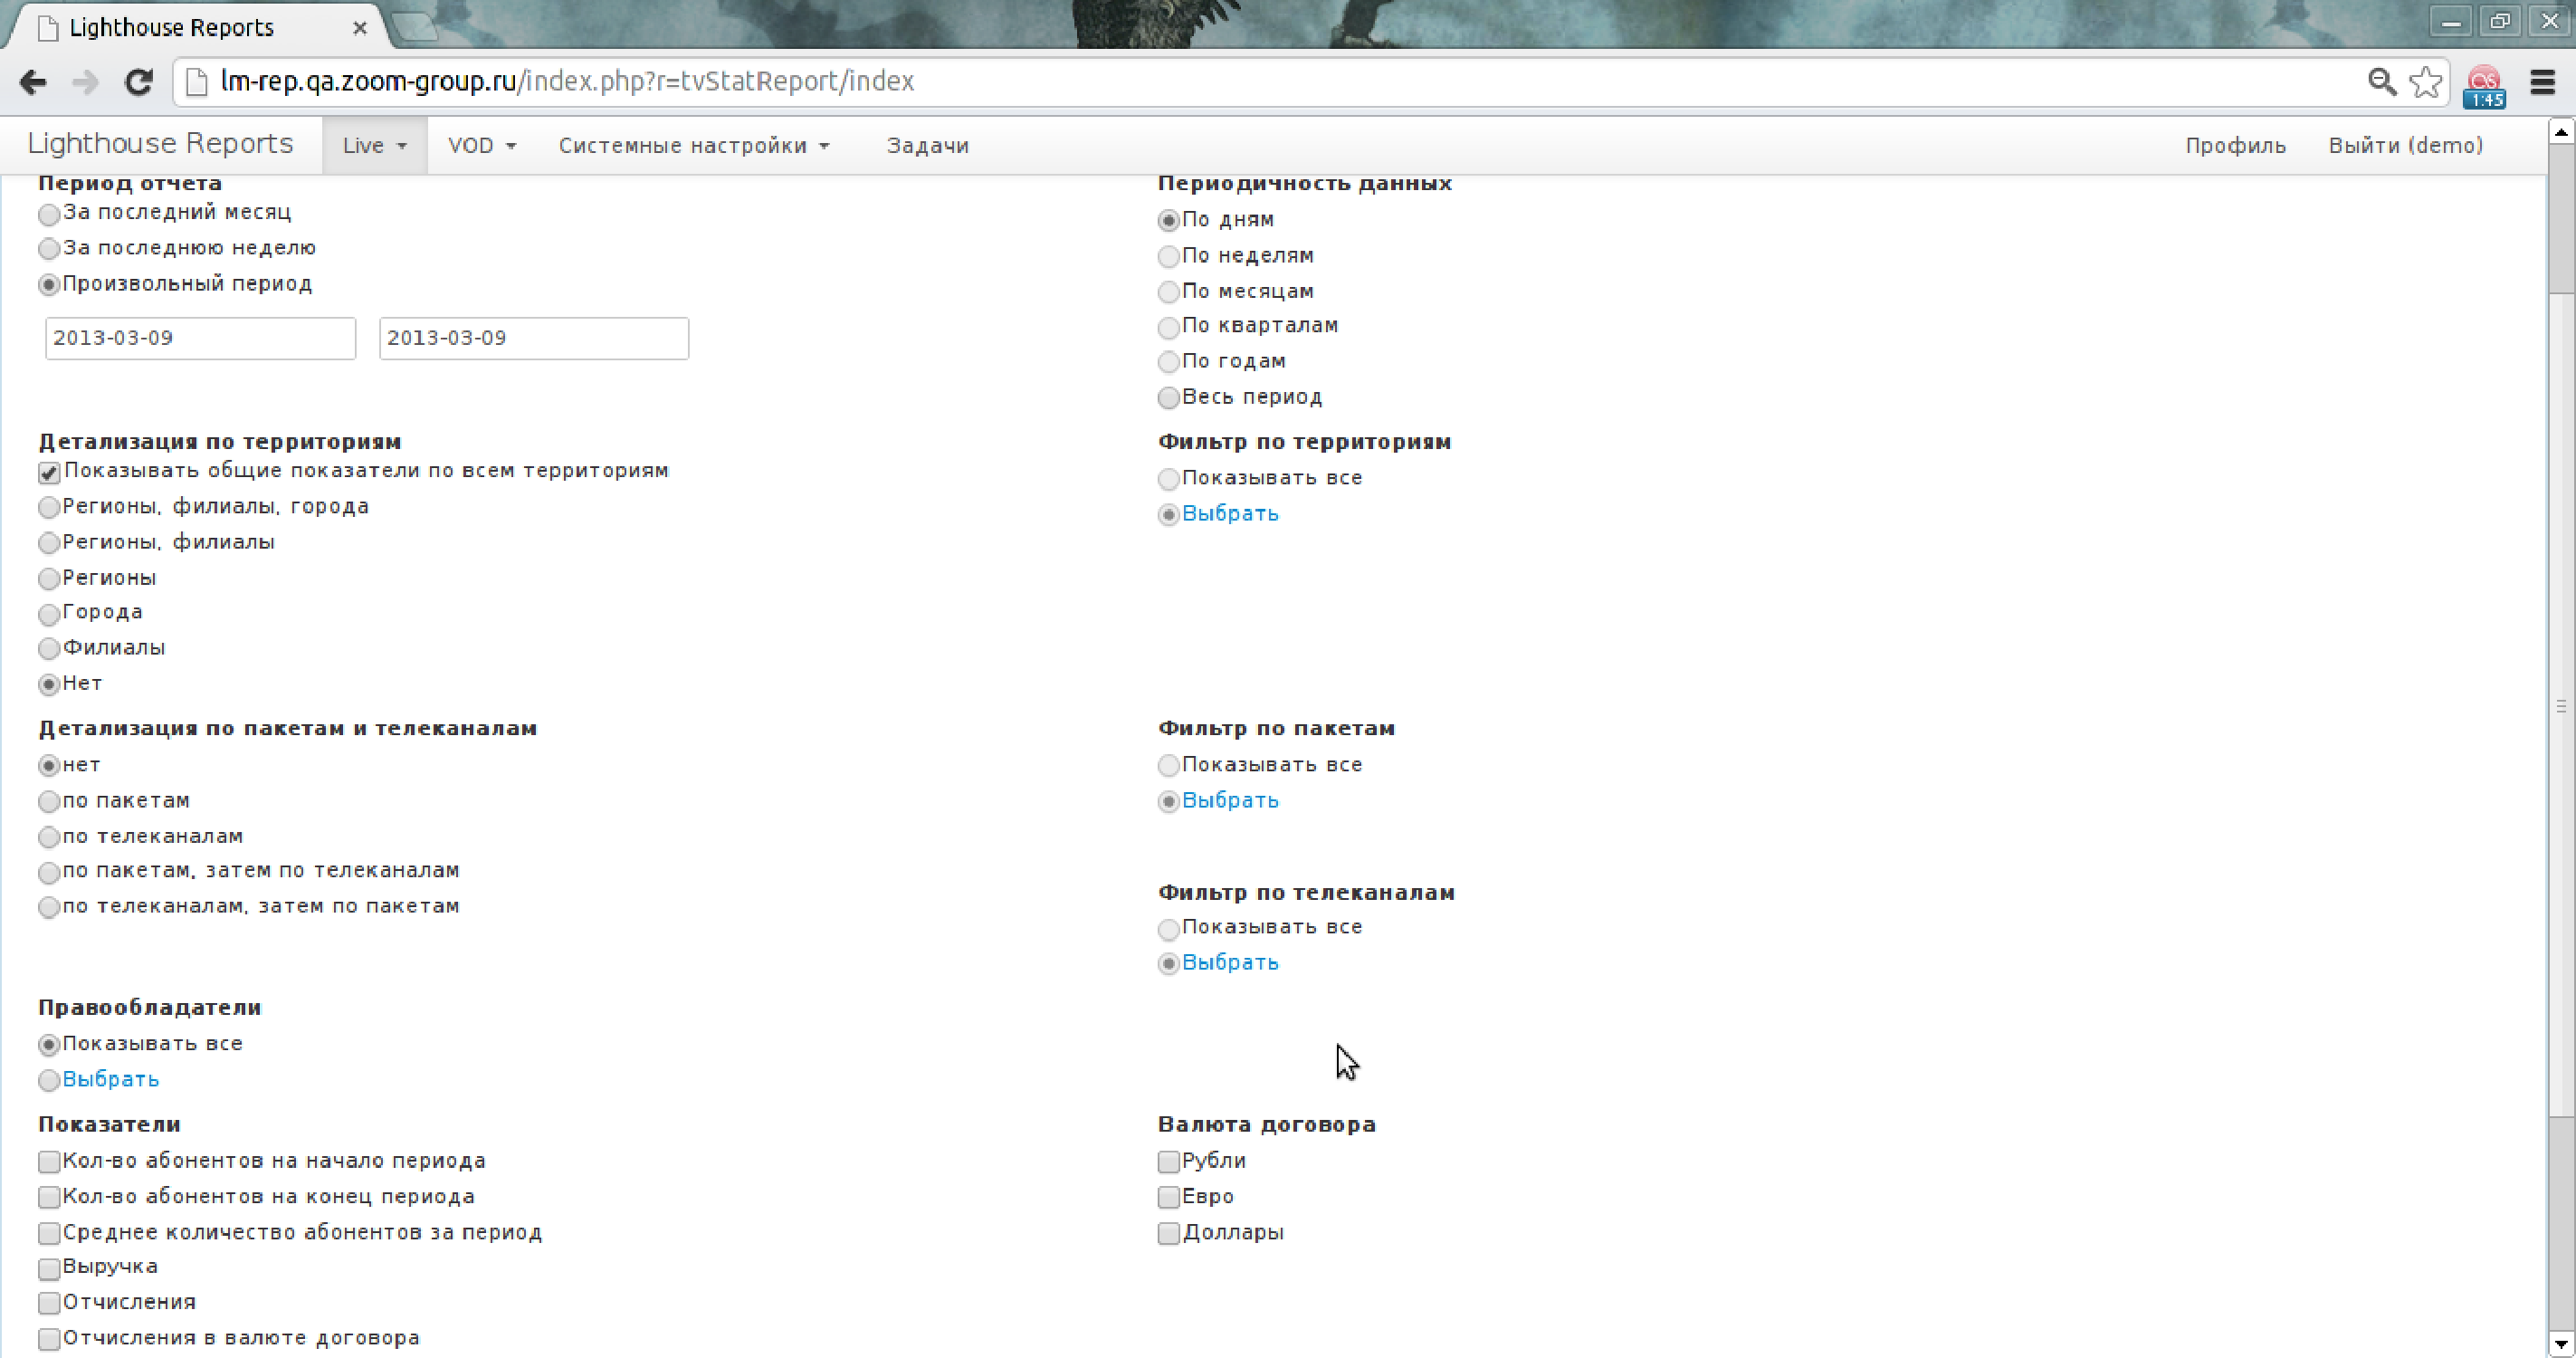
\includegraphics[scale=0.3]{../resources/lm_screen.pdf}
\end{figure}
\end{frame}

\begin{frame}
\frametitle{Реализация. Отчеты}
\begin{figure}
\vspace{-0.5cm}
\hspace*{-1cm} 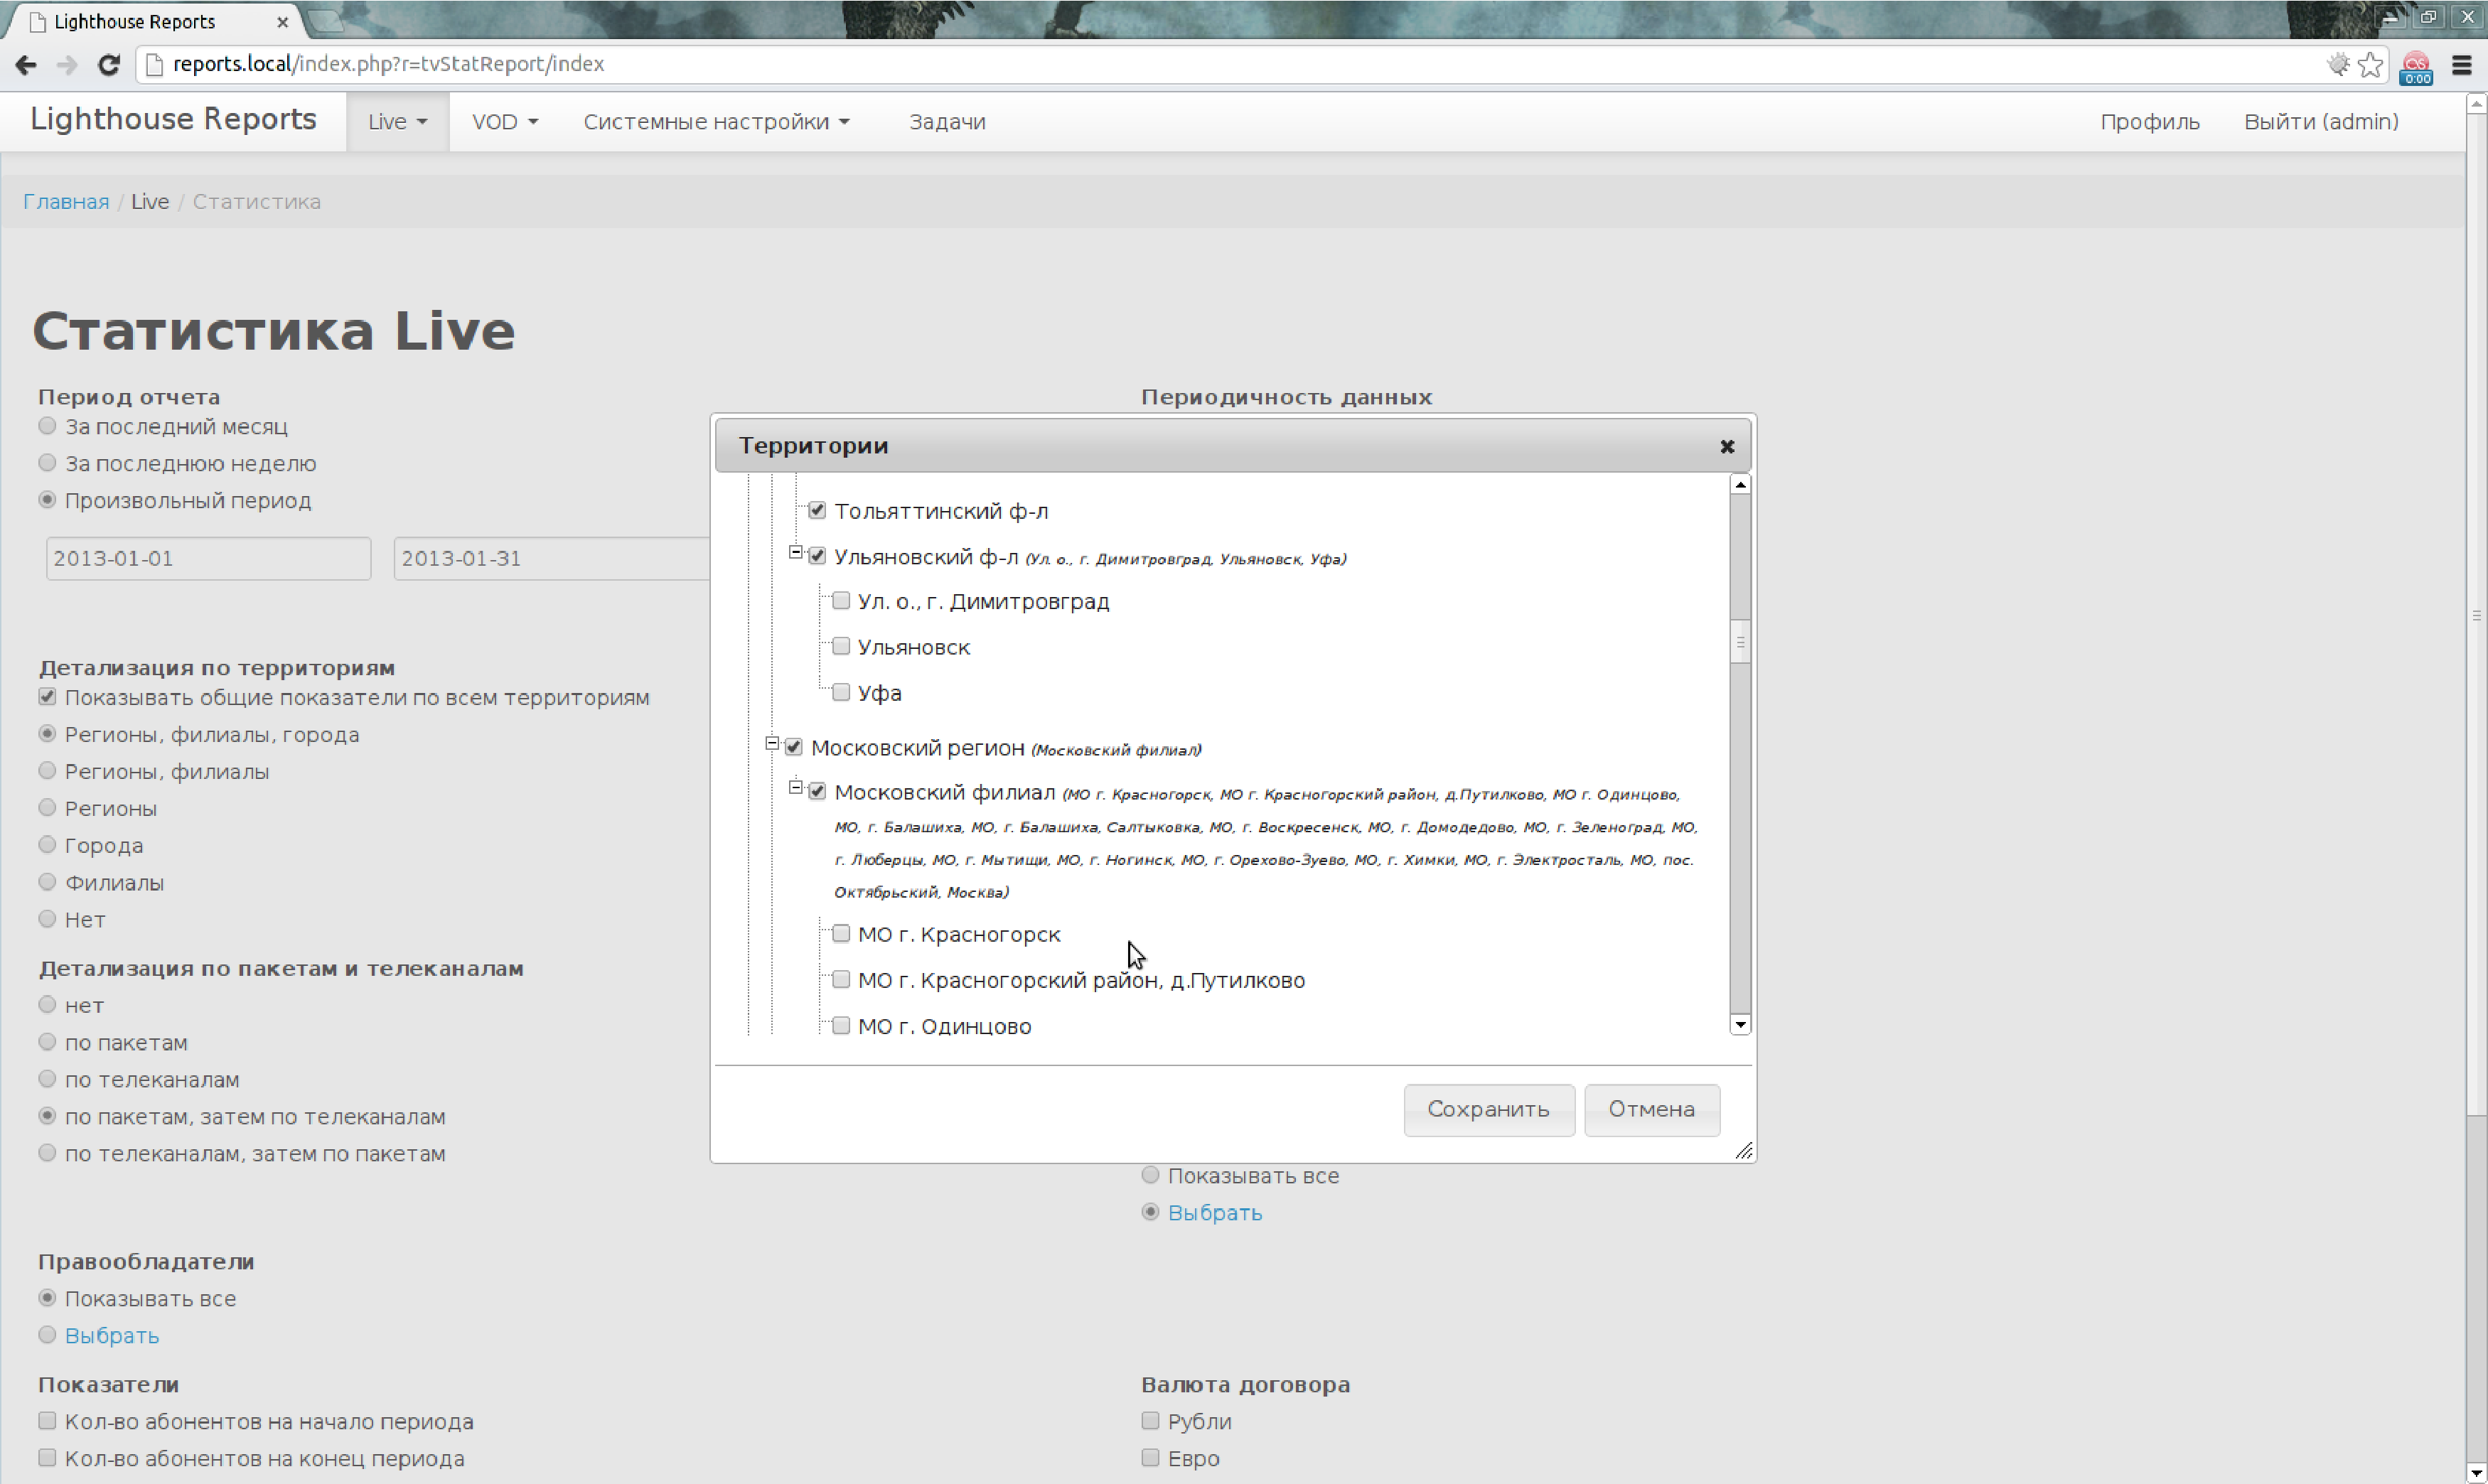
\includegraphics[scale=0.26]{../resources/reports-region.pdf}
\end{figure}
\end{frame}

\begin{frame}
\frametitle{Реализация. Отчеты}
\begin{figure}
\vspace{-0.5cm}
\hspace*{-1cm} 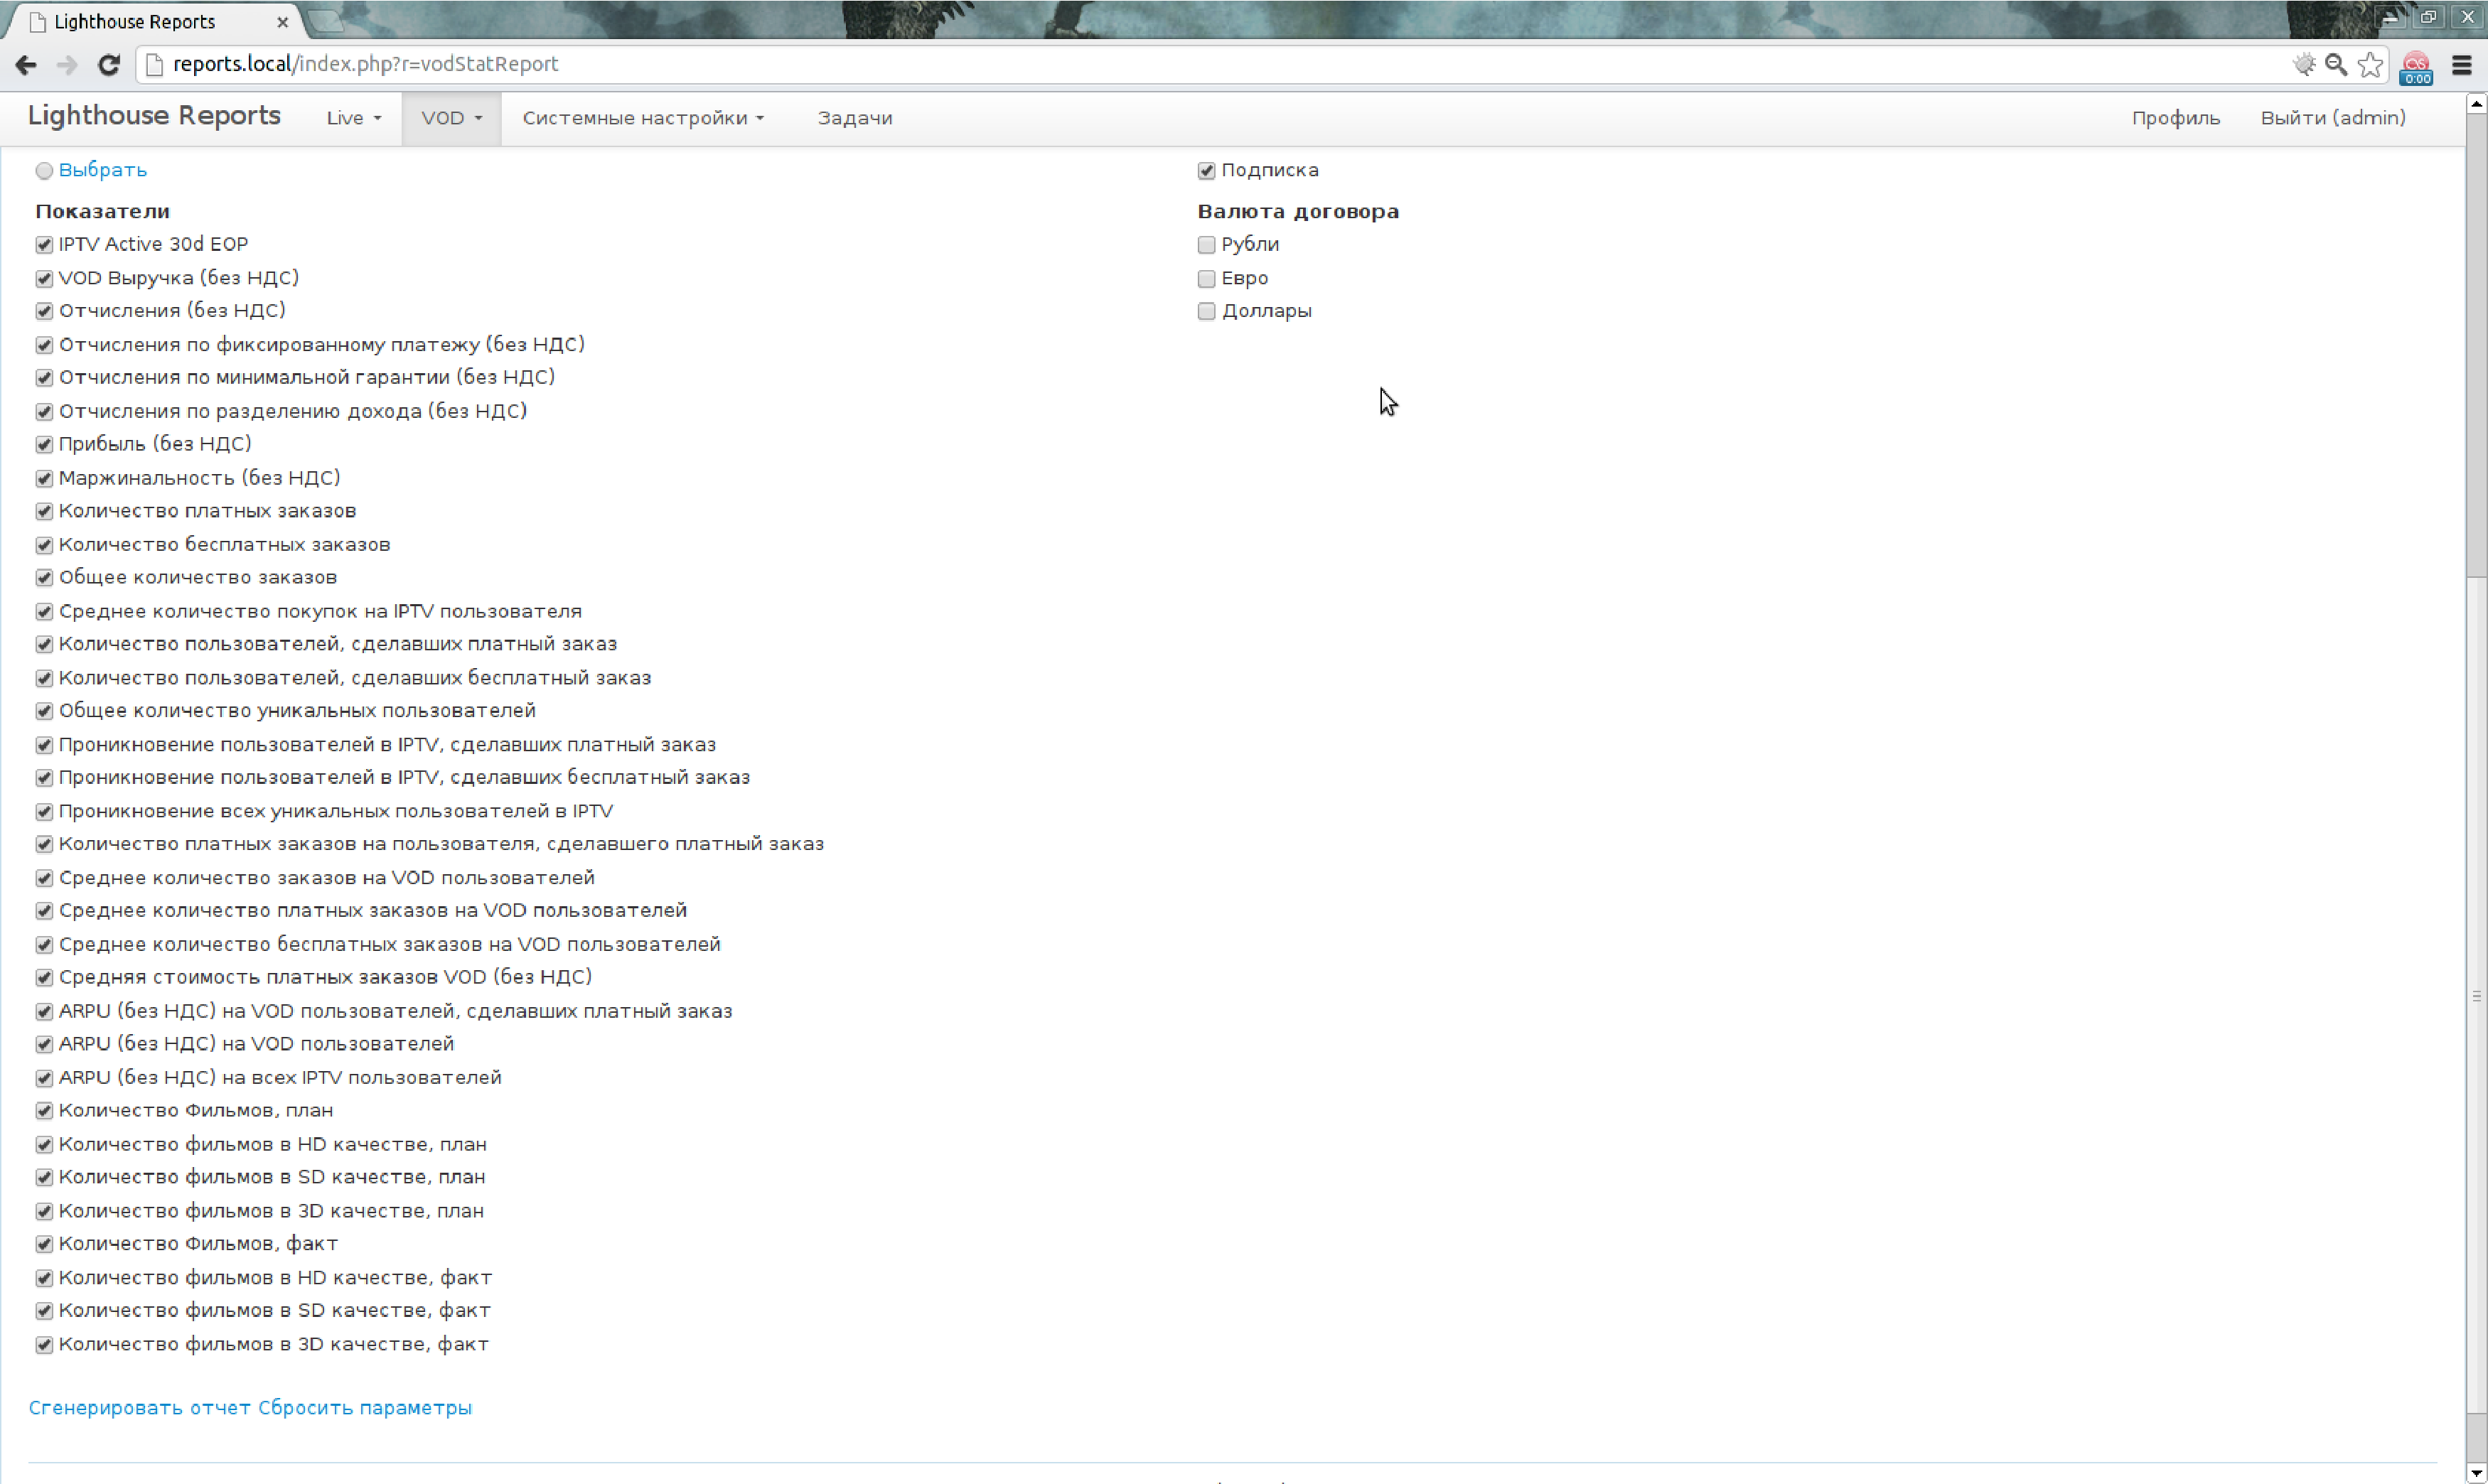
\includegraphics[scale=0.26]{../resources/report-indicator.pdf}
\end{figure}
\end{frame}

\begin{frame}
\frametitle{Реализация. Структура отчета}
\begin{figure}
\vspace{-0.5cm}
\hspace*{-1cm} 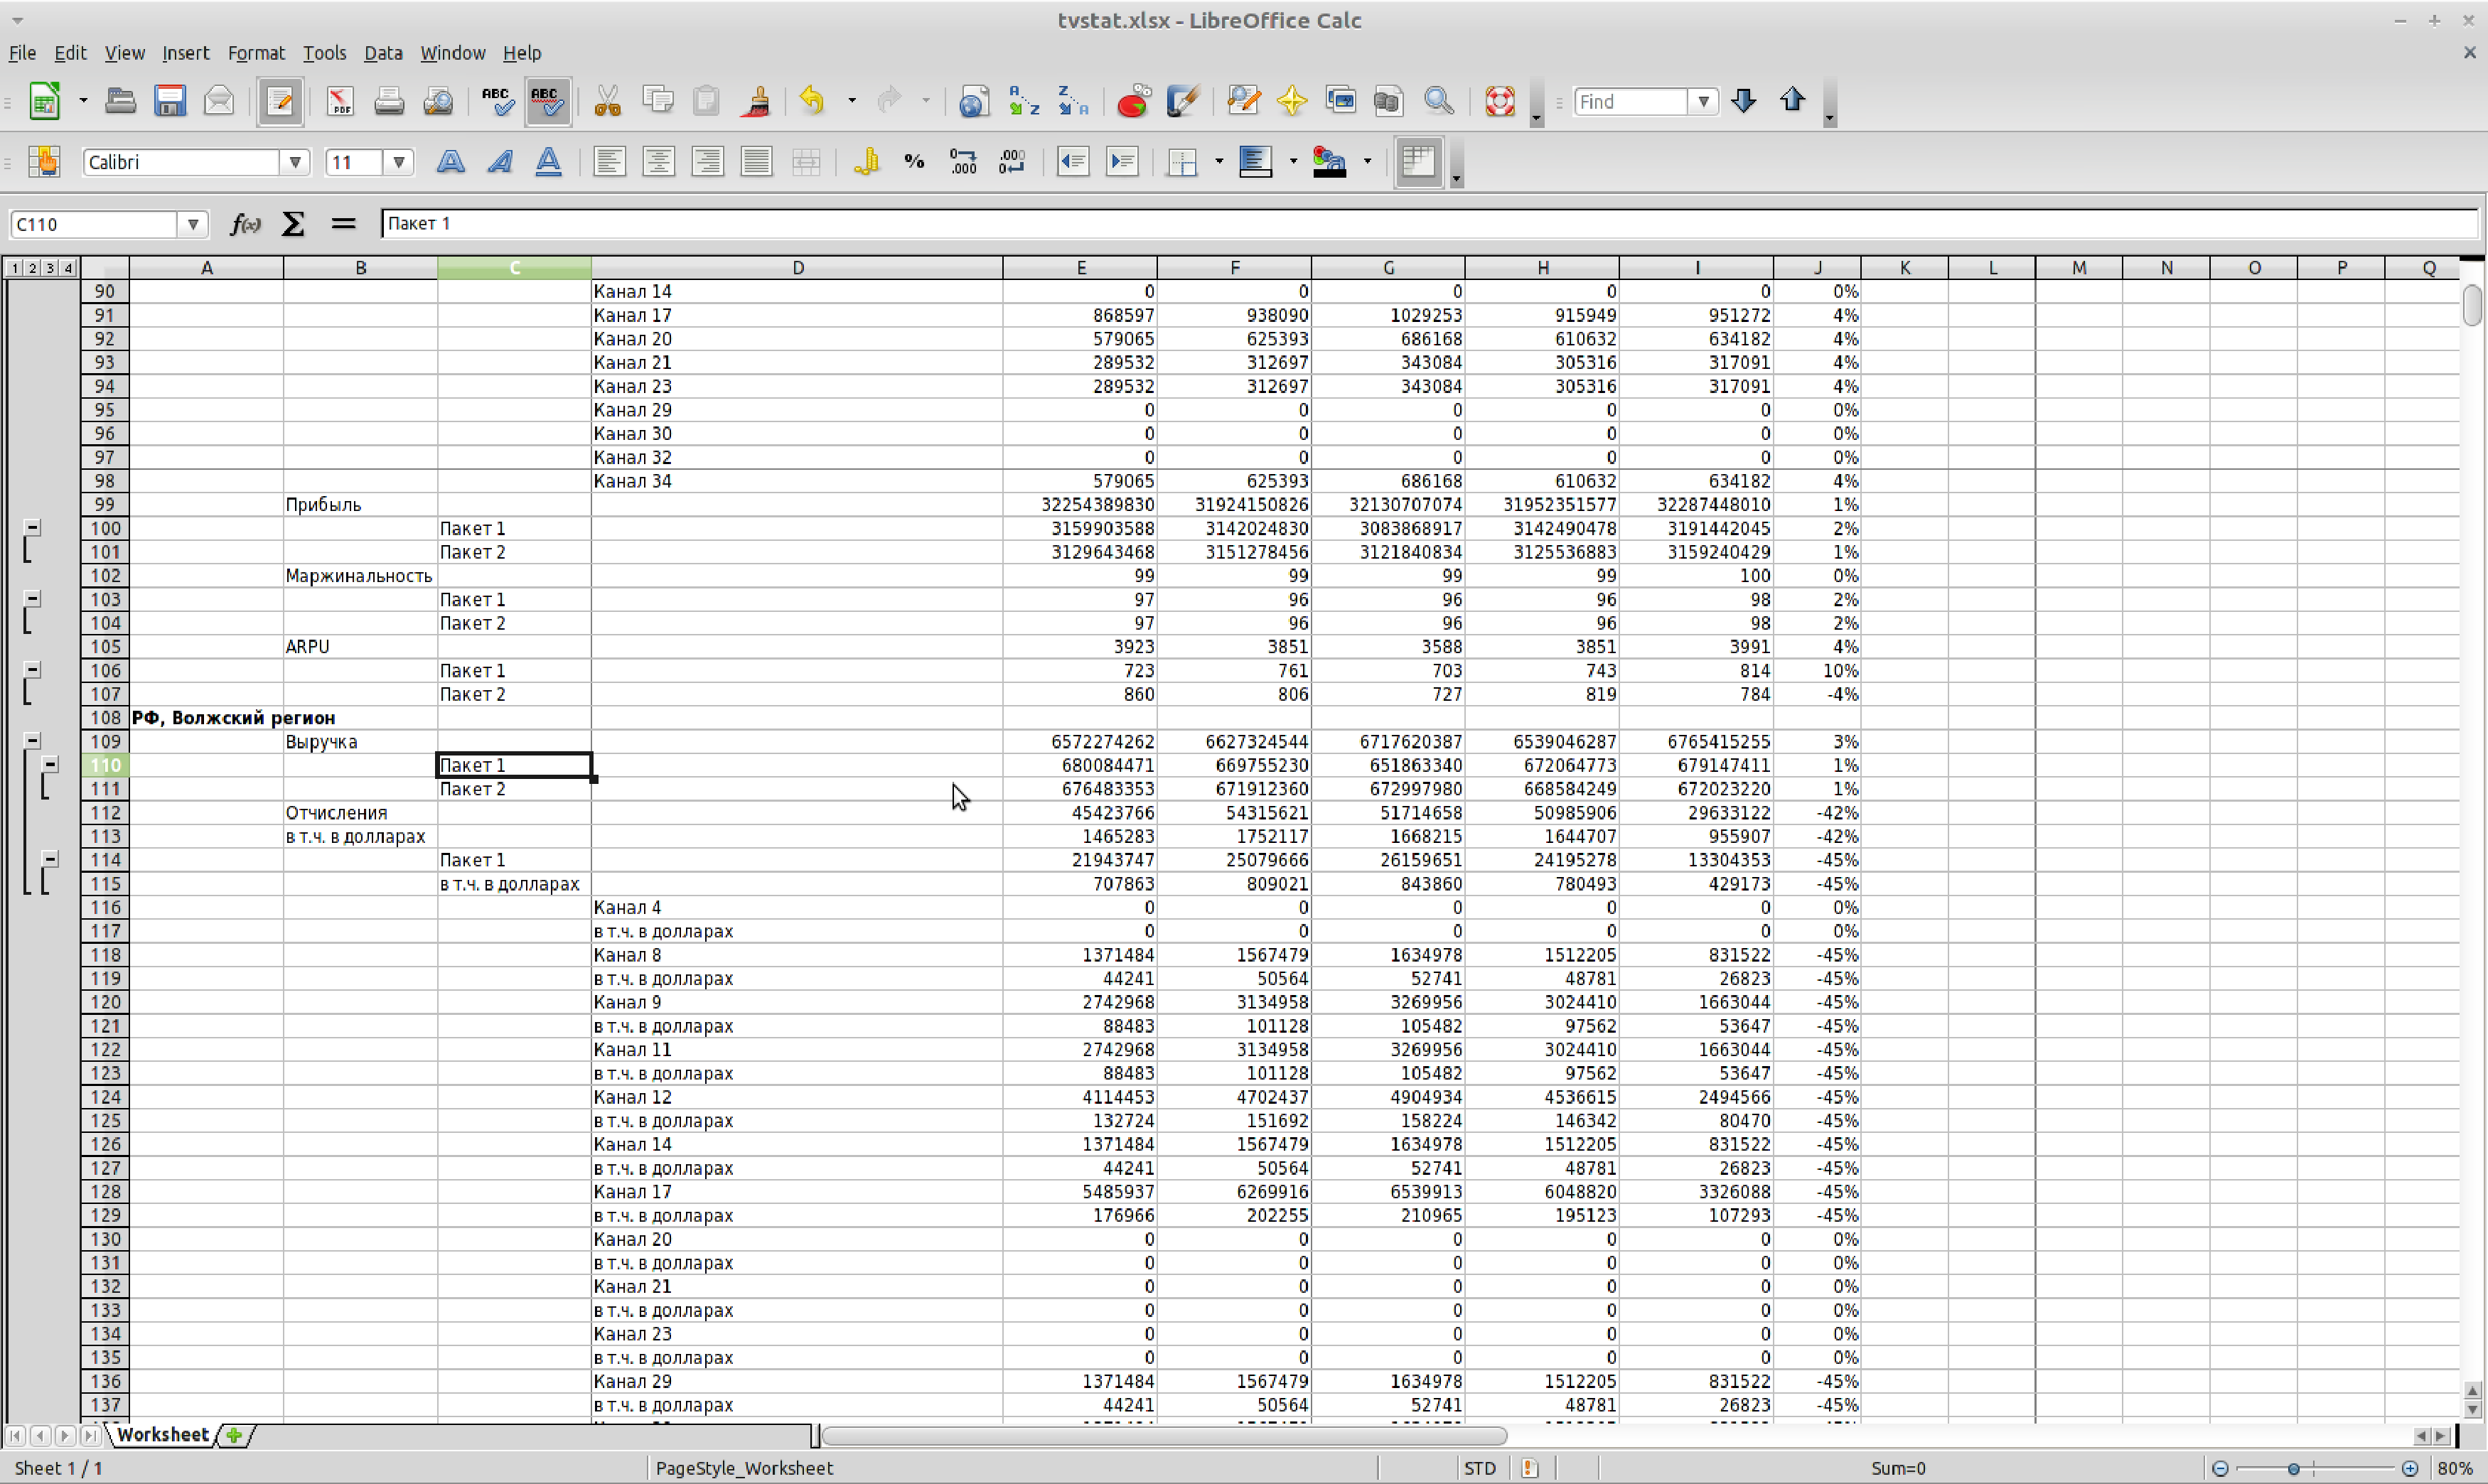
\includegraphics[scale=0.26]{../resources/report1.pdf}
\end{figure}
\end{frame}

\begin{frame}
\frametitle{Реализация. Структура отчета}
\begin{figure}
\vspace{-0.5cm}
\hspace*{-1cm} 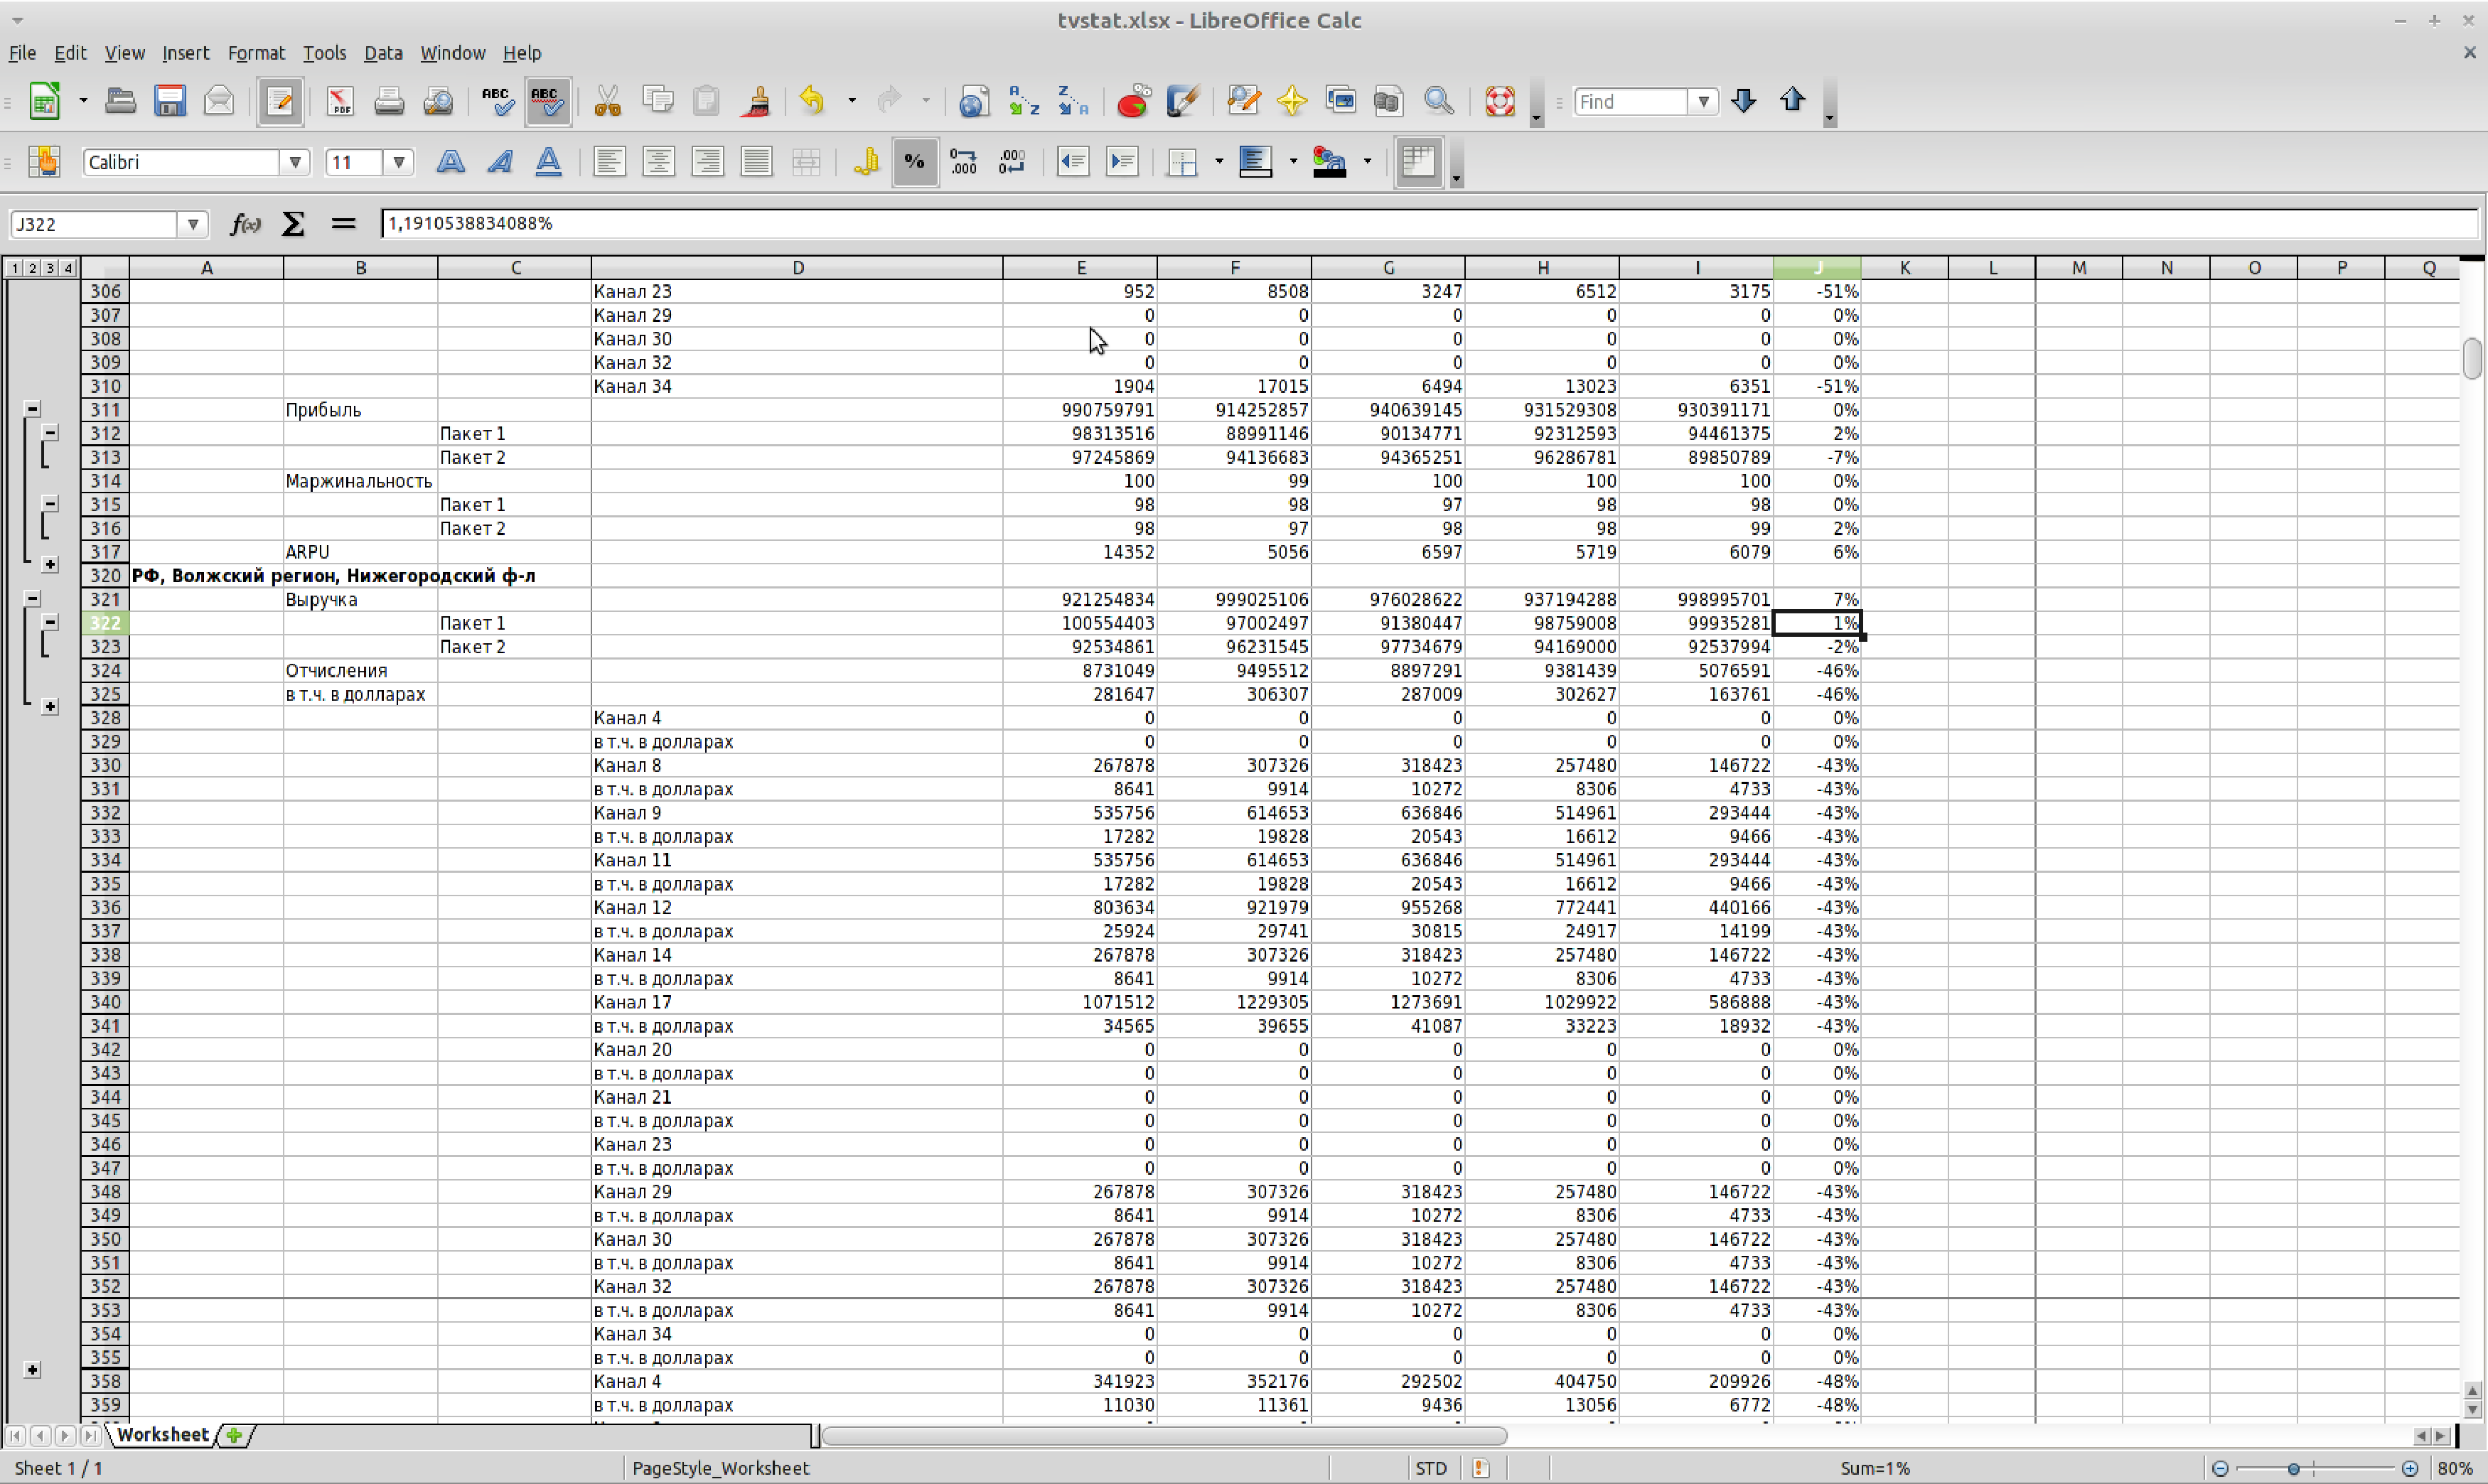
\includegraphics[scale=0.26]{../resources/report2.pdf}
\end{figure}
\end{frame}

\begin{frame}[t]
\frametitle{Реализация. Диаграмма классов пакета StatReport}
\begin{figure}
\begin{center}
\vspace{-1cm}
\hspace*{-1cm} 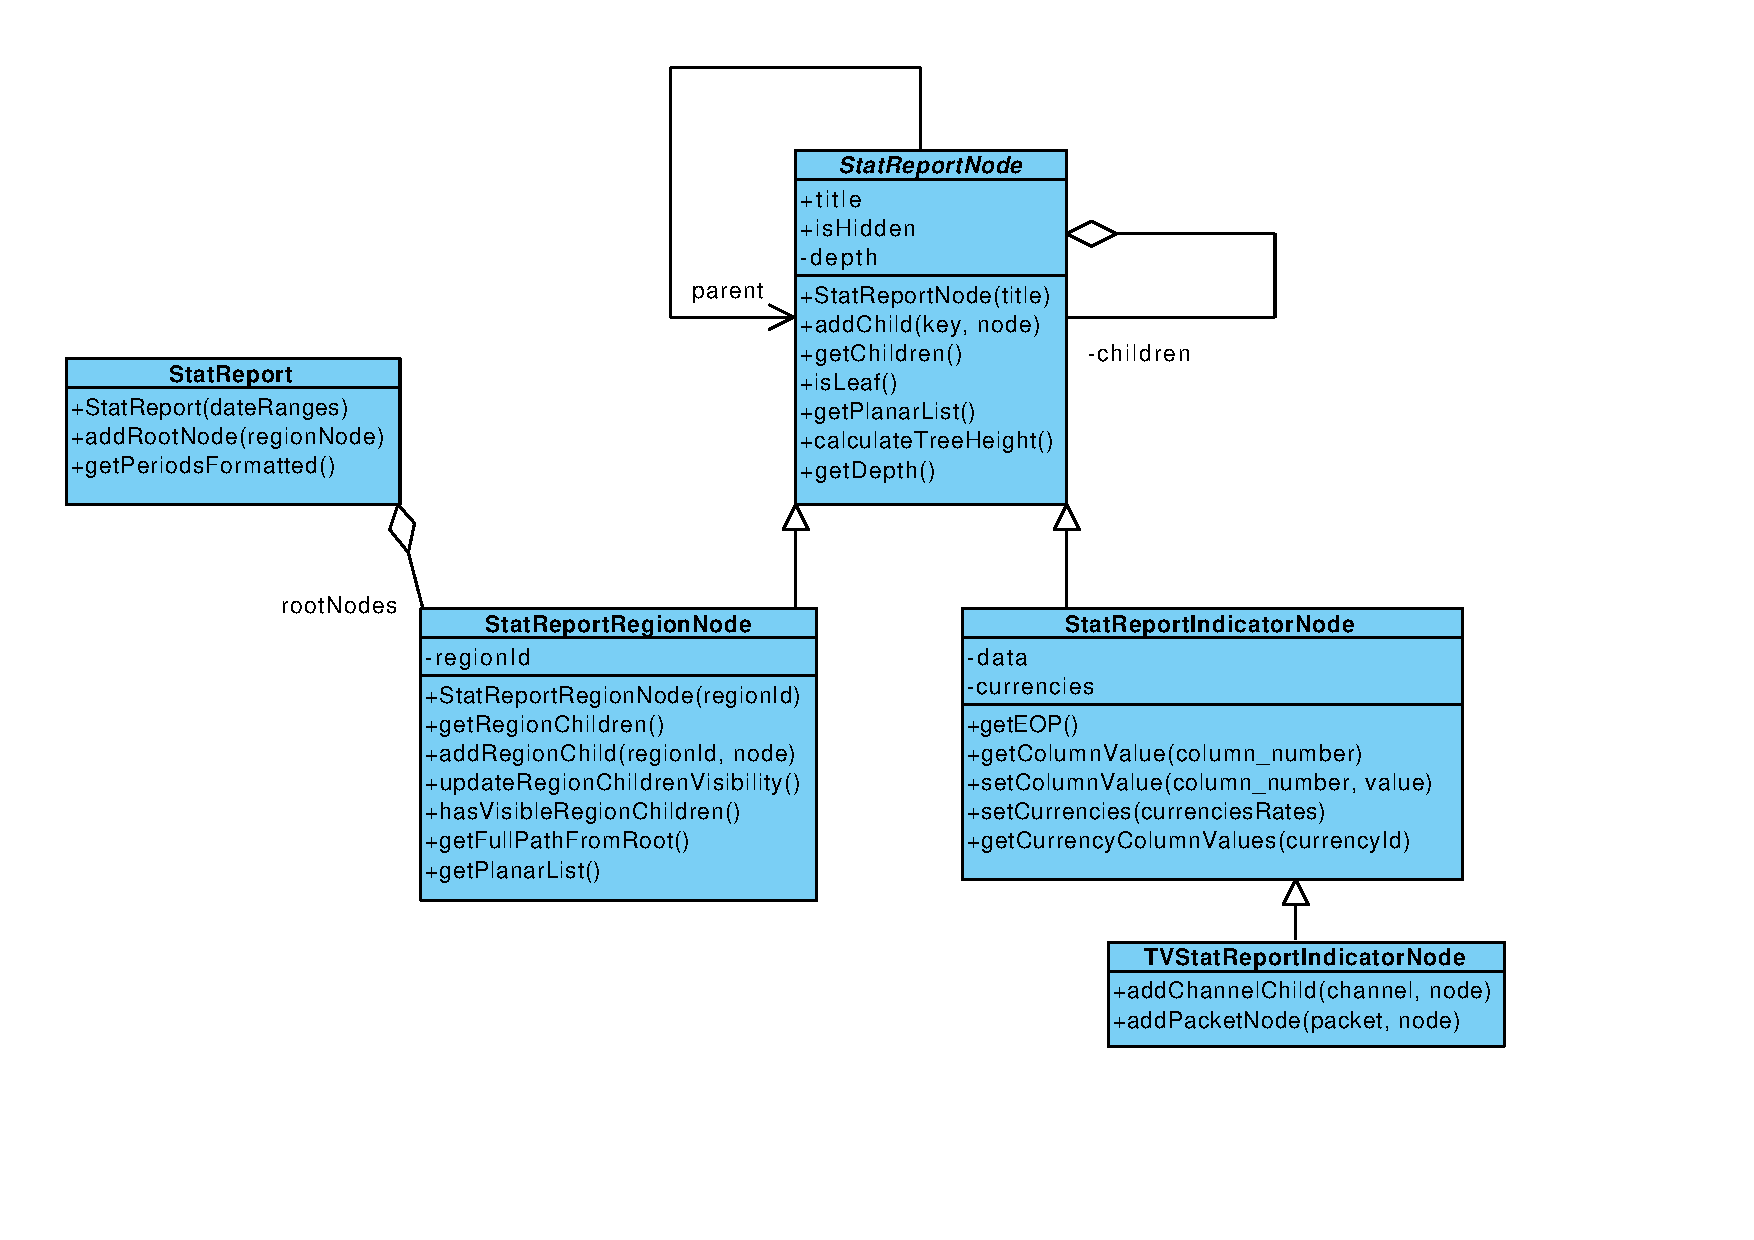
\includegraphics[scale=0.43]{../resources/uml/StatReport.pdf}
\end{center}
\end{figure}
\end{frame}

\begin{frame}[t]
\frametitle{Реализация. Генерация отчета}
\begin{figure}
\begin{center}
\vspace{0cm}
\hspace*{-1cm} 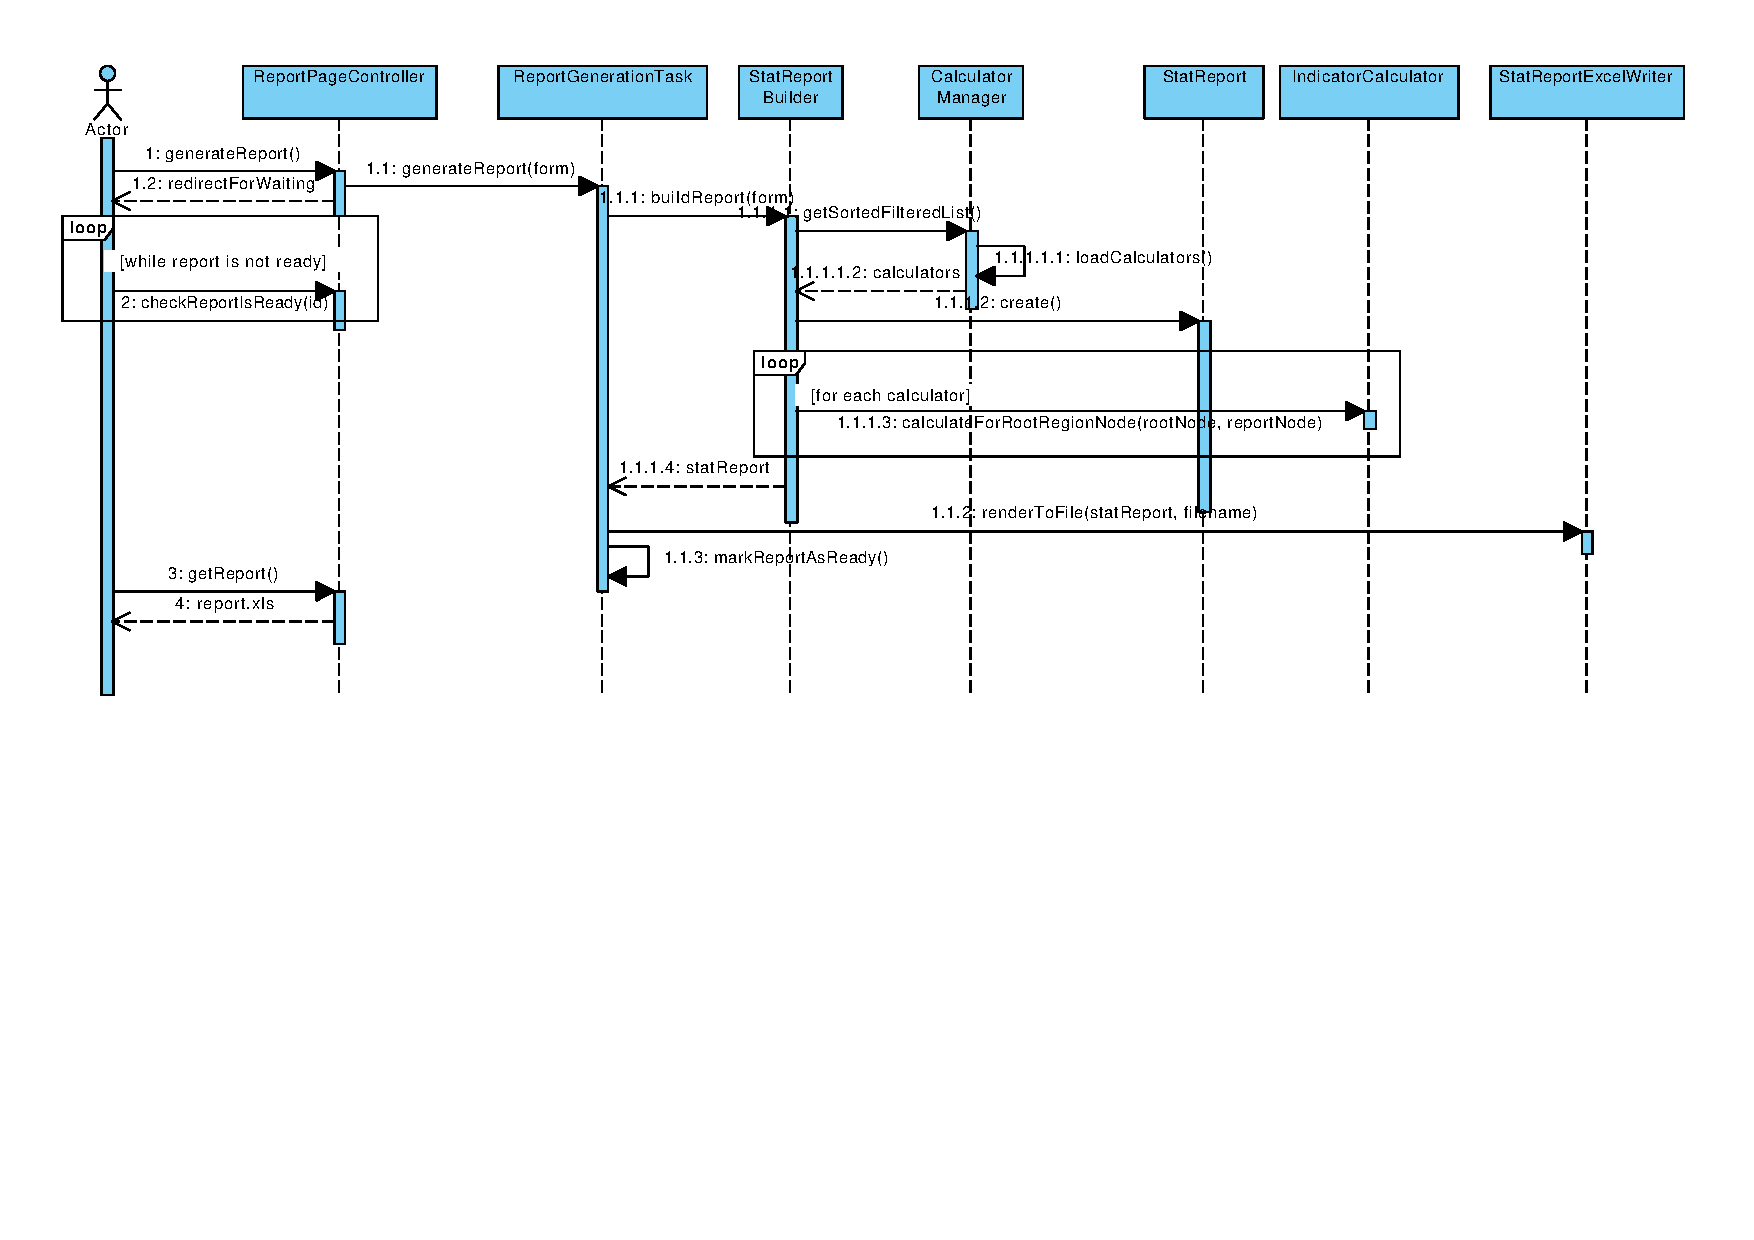
\includegraphics[scale=0.43]{../resources/uml/ReportCreation.pdf}
\end{center}
\end{figure}
\end{frame}

\begin{frame}[t]
\frametitle{Реализация. Загрузка классов-вычислителей показателей}
\begin{figure}
\begin{center}
\vspace{-1cm}
\hspace*{0.5cm} 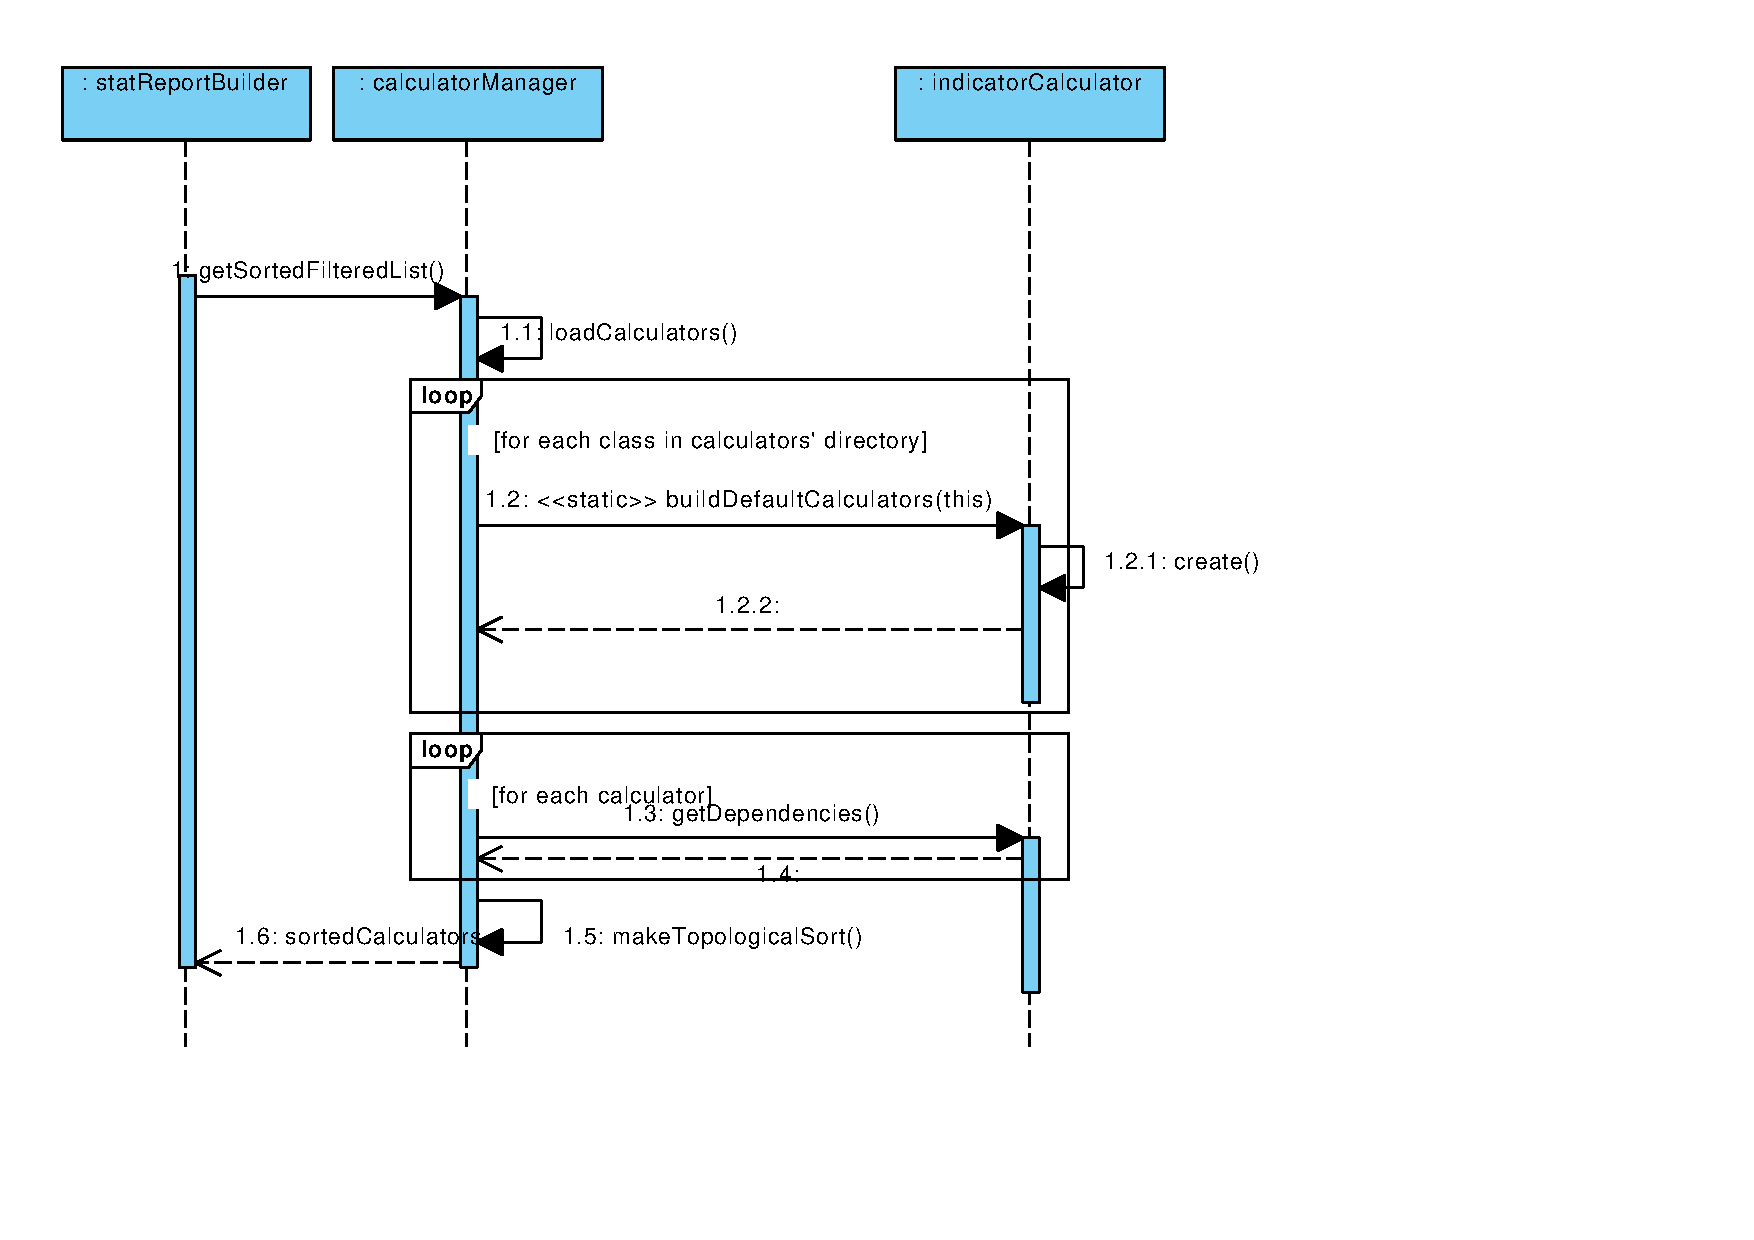
\includegraphics[scale=0.43]{../resources/uml/CalculatorLoading.pdf}
\end{center}
\end{figure}
\end{frame}

\begin{frame}[t]
\frametitle{Реализация. Загрузка классов-вычислителей показателей}
\begin{figure}
\begin{center}
\vspace{0cm}
\hspace*{-1cm} 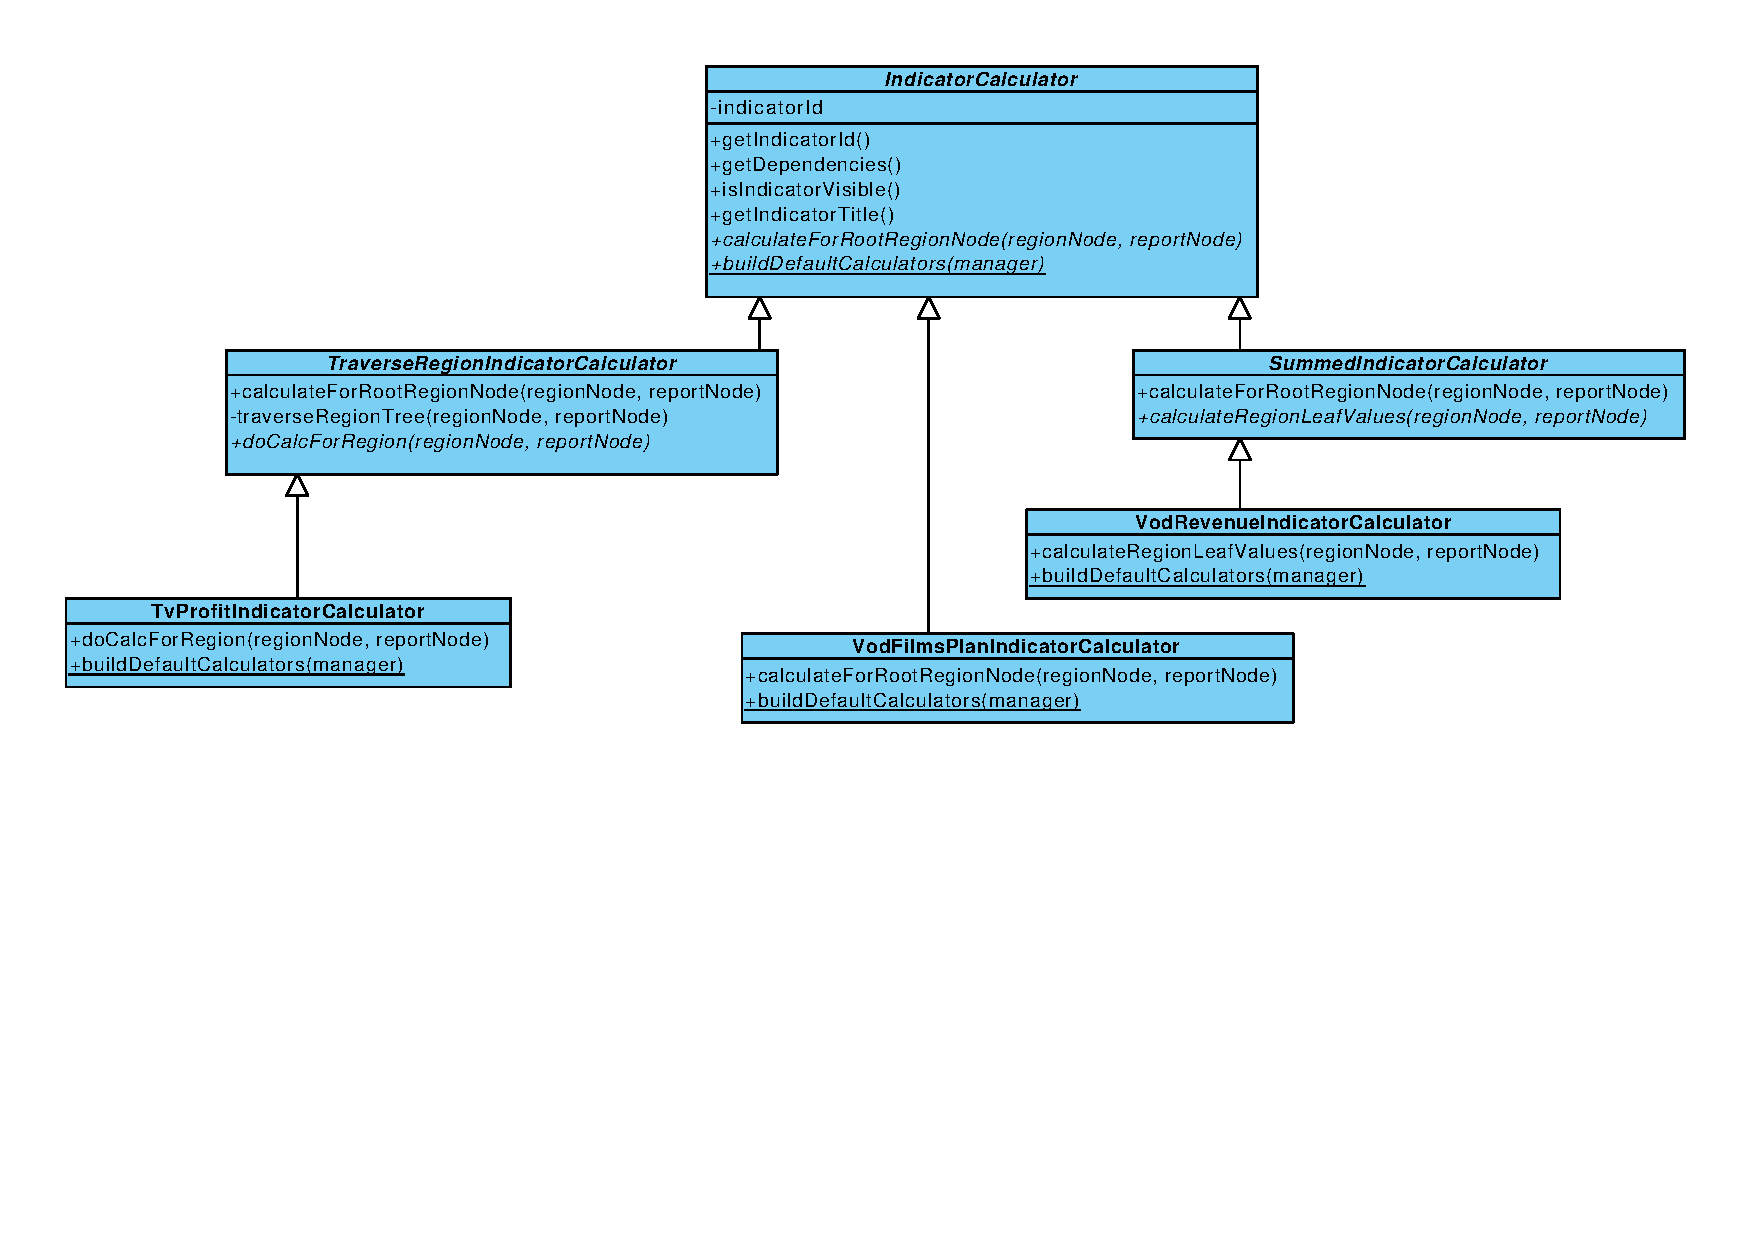
\includegraphics[scale=0.43]{../resources/uml/StatReportIndicatorCalculator.pdf}
\end{center}
\end{figure}
\end{frame}

\begin{frame}
\frametitle{Результаты}
В ходе выполнения ВКР были спроектированы и реализованы:
\begin{enumerate}
\item {
Импорт данных из биллинга провайдера
}
\item {
Страницы поиска и редактирования данных в системе (для более чем 20 типов сущностей)
}
\item {
Расчет отчислений по категории LIVE
}
\item {
Генерация отчетов по LIVE и VOD
}
\end{enumerate}


Система установлена и введена в эксплуатацию

\end{frame}

\begin{frame}
\frametitle{Перспективы дальнейшего развития}
В ходе дальнейших работ планируется:
\begin{enumerate}
\item {
Реализовать графическую интерпретацию отчетов
}
\item {
Сделать возможным просматривать отчет в течение времени его построения
}
\item {
Ускорение генерации отчетов за счет уменьшения количества избыточных данных
}
\end{enumerate}


\end{frame}


\begin{frame}
{\Large Спасибо за внимание!}
\end{frame}

\end{document}
